\documentclass[12pt]{article}

% Packages:
\usepackage{graphicx}
\usepackage[portuguese]{babel}
\usepackage[utf8]{inputenc}
\usepackage{setspace}
\usepackage{listings}
\usepackage{hyperref}
\usepackage{tocloft}
\usepackage{fancyhdr}
\usepackage{placeins}
\usepackage{subcaption}
\usepackage{subfiles}
\usepackage{outlines}
\usepackage{indentfirst}
\usepackage{amsmath}
\usepackage{enumerate}
\usepackage{subfiles}
\usepackage{color, colortbl, xcolor}
\usepackage{multicol}
%---

% Options:
\setstretch{1} % Espaçamento entre linhas
\usepackage[top=3cm, bottom=2cm, left=1.5cm, right=1.5cm]{geometry}
\PassOptionsToPackage{hyphens}{url}
\title{}
\date{}

% Code customization:
% Default fixed font does not support bold face
\DeclareFixedFont{\ttb}{T1}{txtt}{bx}{n}{10} % for bold
\DeclareFixedFont{\ttm}{T1}{txtt}{m}{n}{10}  % for normal

\lstset{
	basicstyle=\footnotesize,
	columns=fullflexible,
    keywordstyle=\ttb\color{blue},
	stringstyle=\ttm\color{green},
	commentstyle=\color{gray},
	frame=None,
	breaklines=true,
	showstringspaces=false,
	postbreak=\mbox{\textcolor{red}{$\hookrightarrow$}\space},
}

%---
% Document:
\begin{document}
	% Cabeçalho:
\begin{figure}
		\begin{minipage}{.3\linewidth}
			\centering
			
\includegraphics[width=.6\linewidth]{imgs/ufpa.jpg}
		\end{minipage}
		\begin{minipage}{.70\linewidth}
			\flushleft
			\paragraph{}
			\textbf{ }\newline
			\textbf{UNIVERSIDADE FEDERAL DO PARÁ} \newline
			\textbf{INSTITUTO DE TECNOLOGIA} \newline
			\textbf{FACULDADE DE ENGENHARIA DA COMPUTAÇÃO E TELECOMUNICAÇÕES} \newline
			\textbf{TE05205 - Top. Especiais em Engenharia de Computação II} \newline
            \textbf{Prof. Dr. Roberto Celio Limão de Oliveira} \newline
            \textbf{Aluna: Camila Novaes Silva (201606840055)}
		\end{minipage}
\end{figure}
\FloatBarrier
\begin{center}
    {\Large \textbf{Atividade 04 - Função F6 elevada}}
\end{center}
%%%%%%%%%%%%%
\hfill

O Algoritmo genético (AG) descrito a seguir foi implementado para solucionar um exemplo
de otimização, especificamente o de maximização da função $f6$ elevada, de duas variáveis.
A função a ser maximizada é
$$f(x,y) = 999.5 - \frac{[\sin(\sqrt{(x^2 + y^2)})]^2 - 0.5}{[1 + 0.001(x^2 + y^2)]^2}$$.

% trim: left lower right upper

Assim, o objetivo é encontrar o valor de $x$,$y \in [-100,100]$ que maximiza a função $f$.

\begin{enumerate}[(a)]
	\item Representação
		\subitem Para representar todos os valores dentro do intervalo $[-100,100]$, com uma precisão
		de 5 casa decimais foram necessários 25 bits para cada variável, totalizando 50 bits para cada cromossomo.
		\subitem Para a decodificação entre real e binário foram utilizadas as seguintes equações:
		$$x_{real} = d(x') =  -100 + x' * \frac{200}{2^{25} - 1}$$
		$$y_{real} = d(y') =  -100 + y' * \frac{200}{2^{25} - 1}$$
		\subitem Onde $x'$, $y'$ são a conversão direta da base binária para a decimal.

	\item Seleção
		\subitem Foram utilizados dois algoritimos de seleção, a roleta proporcional ao fitness com e
		sem normalização linear. No caso da normalização linear, o cromossomo será avaliado utilizando
		um novo valor de aptidão, utilizando a seguinte forma:
		$$A_i = min - \frac{(max - min)}{pop\_size - 1}*(i - 1), i \in [1, pop\_size]$$

		onde, o valor $min$ e $max$ podem ser ajustados para aumentar ou diminuir a presão seletiva do algoritimo.
		O relatório apresenta os resultados obtidos com
		ambos dos métodos, uma vez que para o caso da função f6 elevada, o efeito da seleção
		proporcional ao fitness sem normalização é quase nulo porque que as avaliações estão muito próximas.

	\item Operadores genéticos
		\subitem Para realizar o cruzamento, foi utilizado o algoritmo ponto de corte, com apenas um ponto,
		com uma taxa de cruzamento de 75\%. E para a mutação foi utilizada uma taxa igual a 1\%.
	\item Critério de paragem
		\subitem O critério de paragem foi 100 gerações.
\end{enumerate}

Os resultados obtidos são apresentados a seguir. Para a avaliação de performance do algoritimo, foram
realizado os 5 testes, onde cada teste é composto por 50 experimentos, por fim foi calculado a média
dos testes e esse representa o valor final considerado.

Dessa forma, primeiramente foi utilizado seleção proporcional ao fitness sem normalização linear. O resultado obtido
foi a incapacidade de evolução do algoritimo uma vez que as avaliações de todos os cromossomos estão
muito próximas, fazendo com que a seleção não consiga identificar as regiões promissoras (melhores cromossomos). O
resultado desse método é apresentado na tabela~\ref{tab:f6_prop}.

\begin{table}[htb]
	\centering
	\begin{tabular}{|c|c|c|}
		\hline
		\rowcolor[HTML]{9B9B9B}
		Teste & Média do melhor indíviduo & Média da população \\\hline
		1 & 999.75554 & 999.50211 \\\hline
		2 & 999.73148 & 999.50415 \\\hline
		3 & 999.77426 & 999.50371 \\\hline
		4 & 999.74258 & 999.50239 \\\hline
		5 & 999.73780 & 999.50281 \\\hline
		Média Final & 999.74833 & 999.50303 \\\hline
	\end{tabular}
	\caption{Resultados da função f6 elevada utilizando seleção
	proporcional ao fitness sem normalização linear \label{tab:f6_prop}}
\end{table}

\begin{figure}[htb]
	\begin{subfigure}{.45\textwidth}
		\centering
		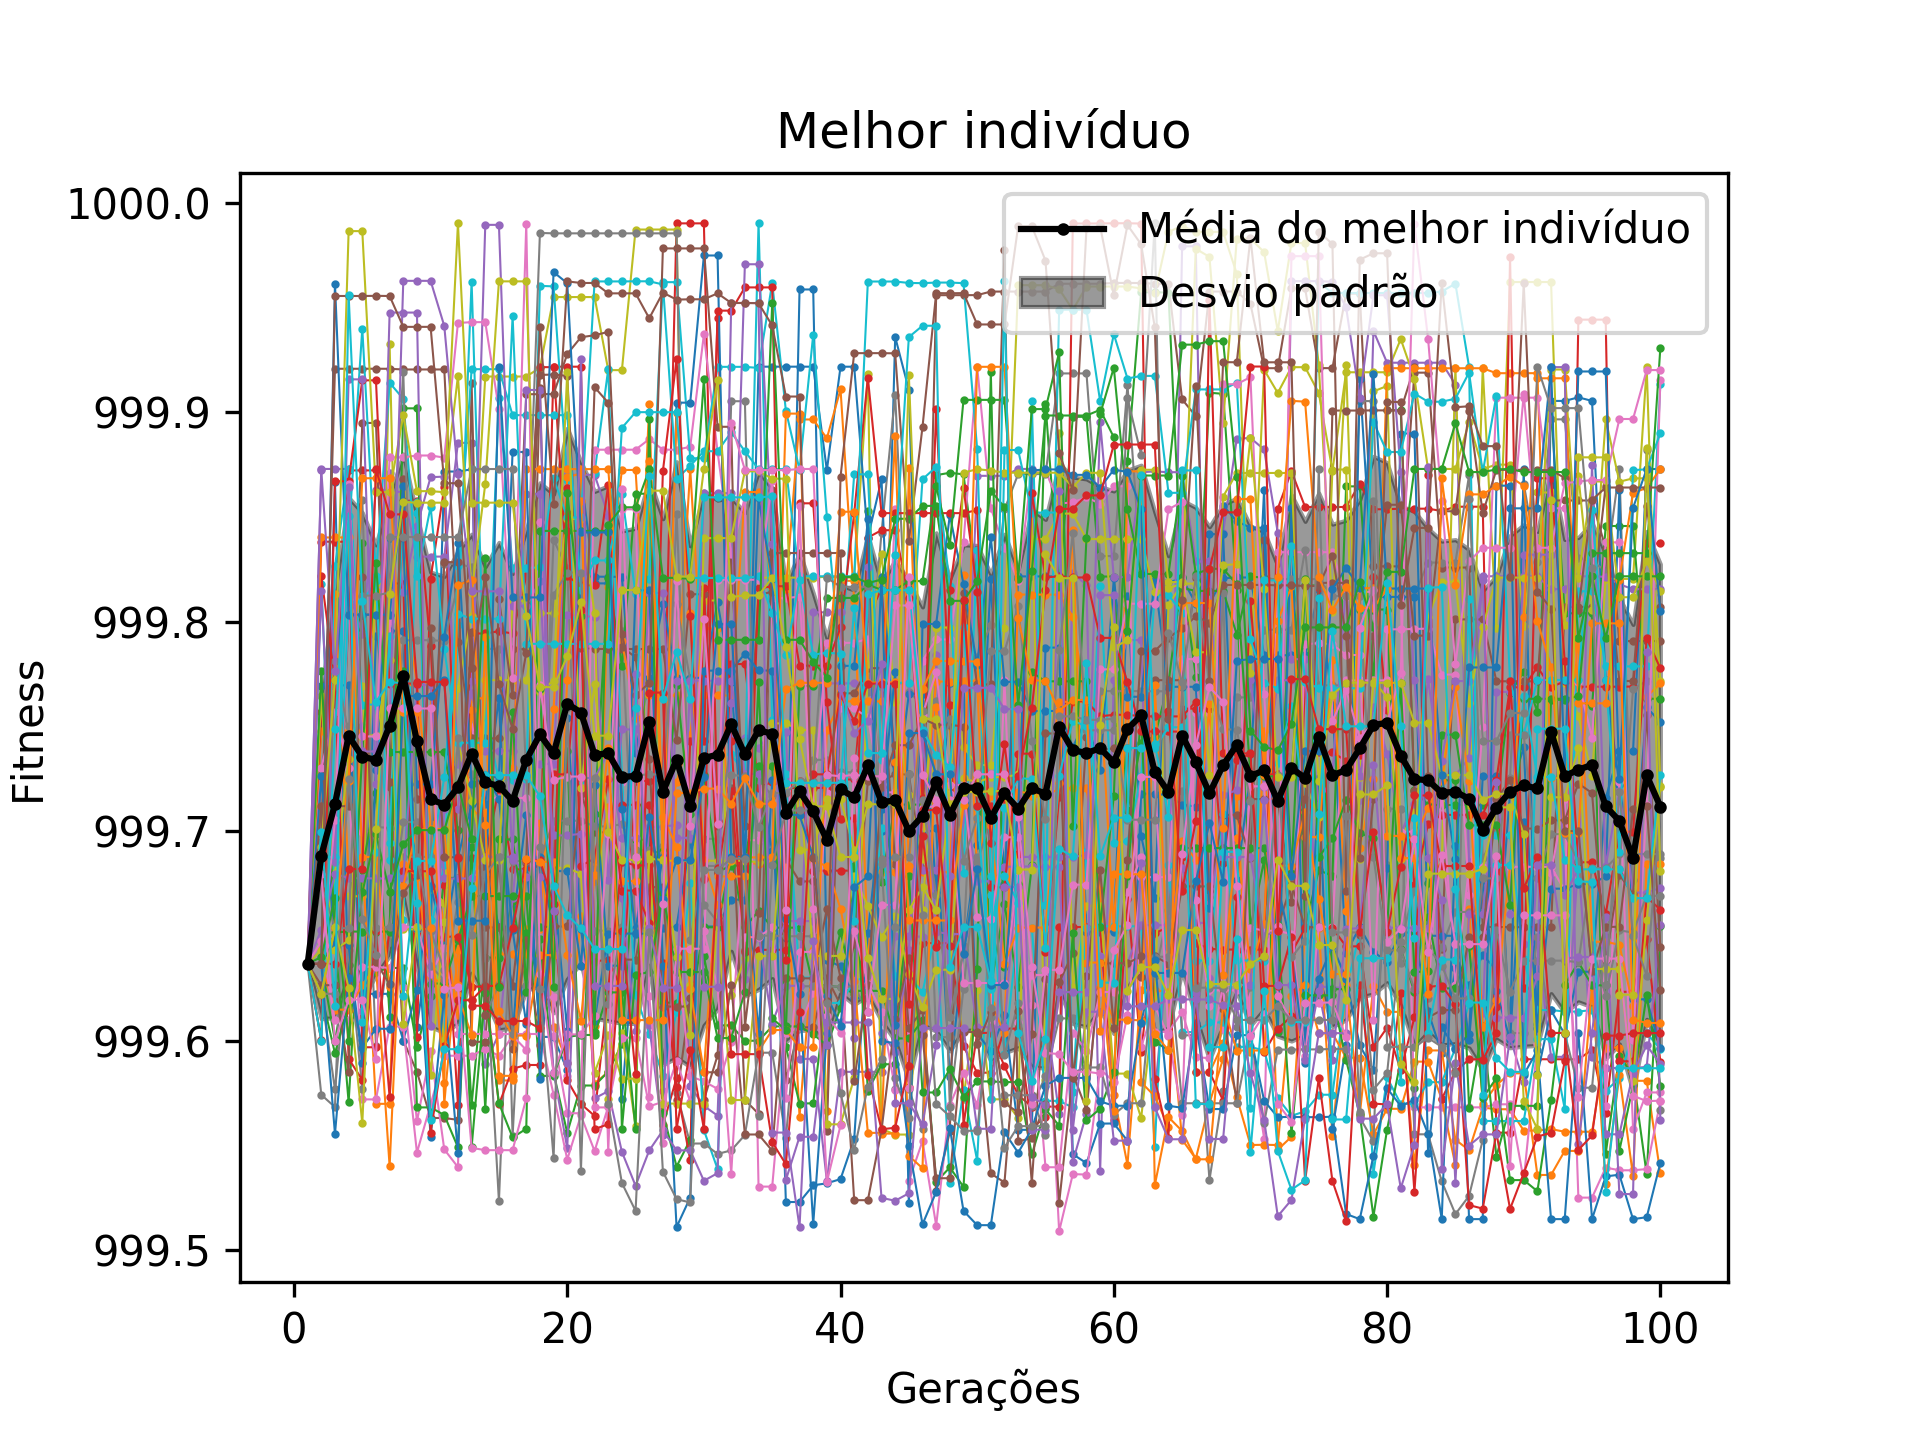
\includegraphics[width=1\textwidth]{./imgs/f6_prop/fitness_vs_gen_best.png}
		\caption{Melhores indíviduos de todos os experimentos ao longo das gerações.
		Em preto é mostrado o comportamento médio dos 50 experimentos. }
	\end{subfigure}
	\hfill
	\begin{subfigure}{.45\textwidth}
		\centering
		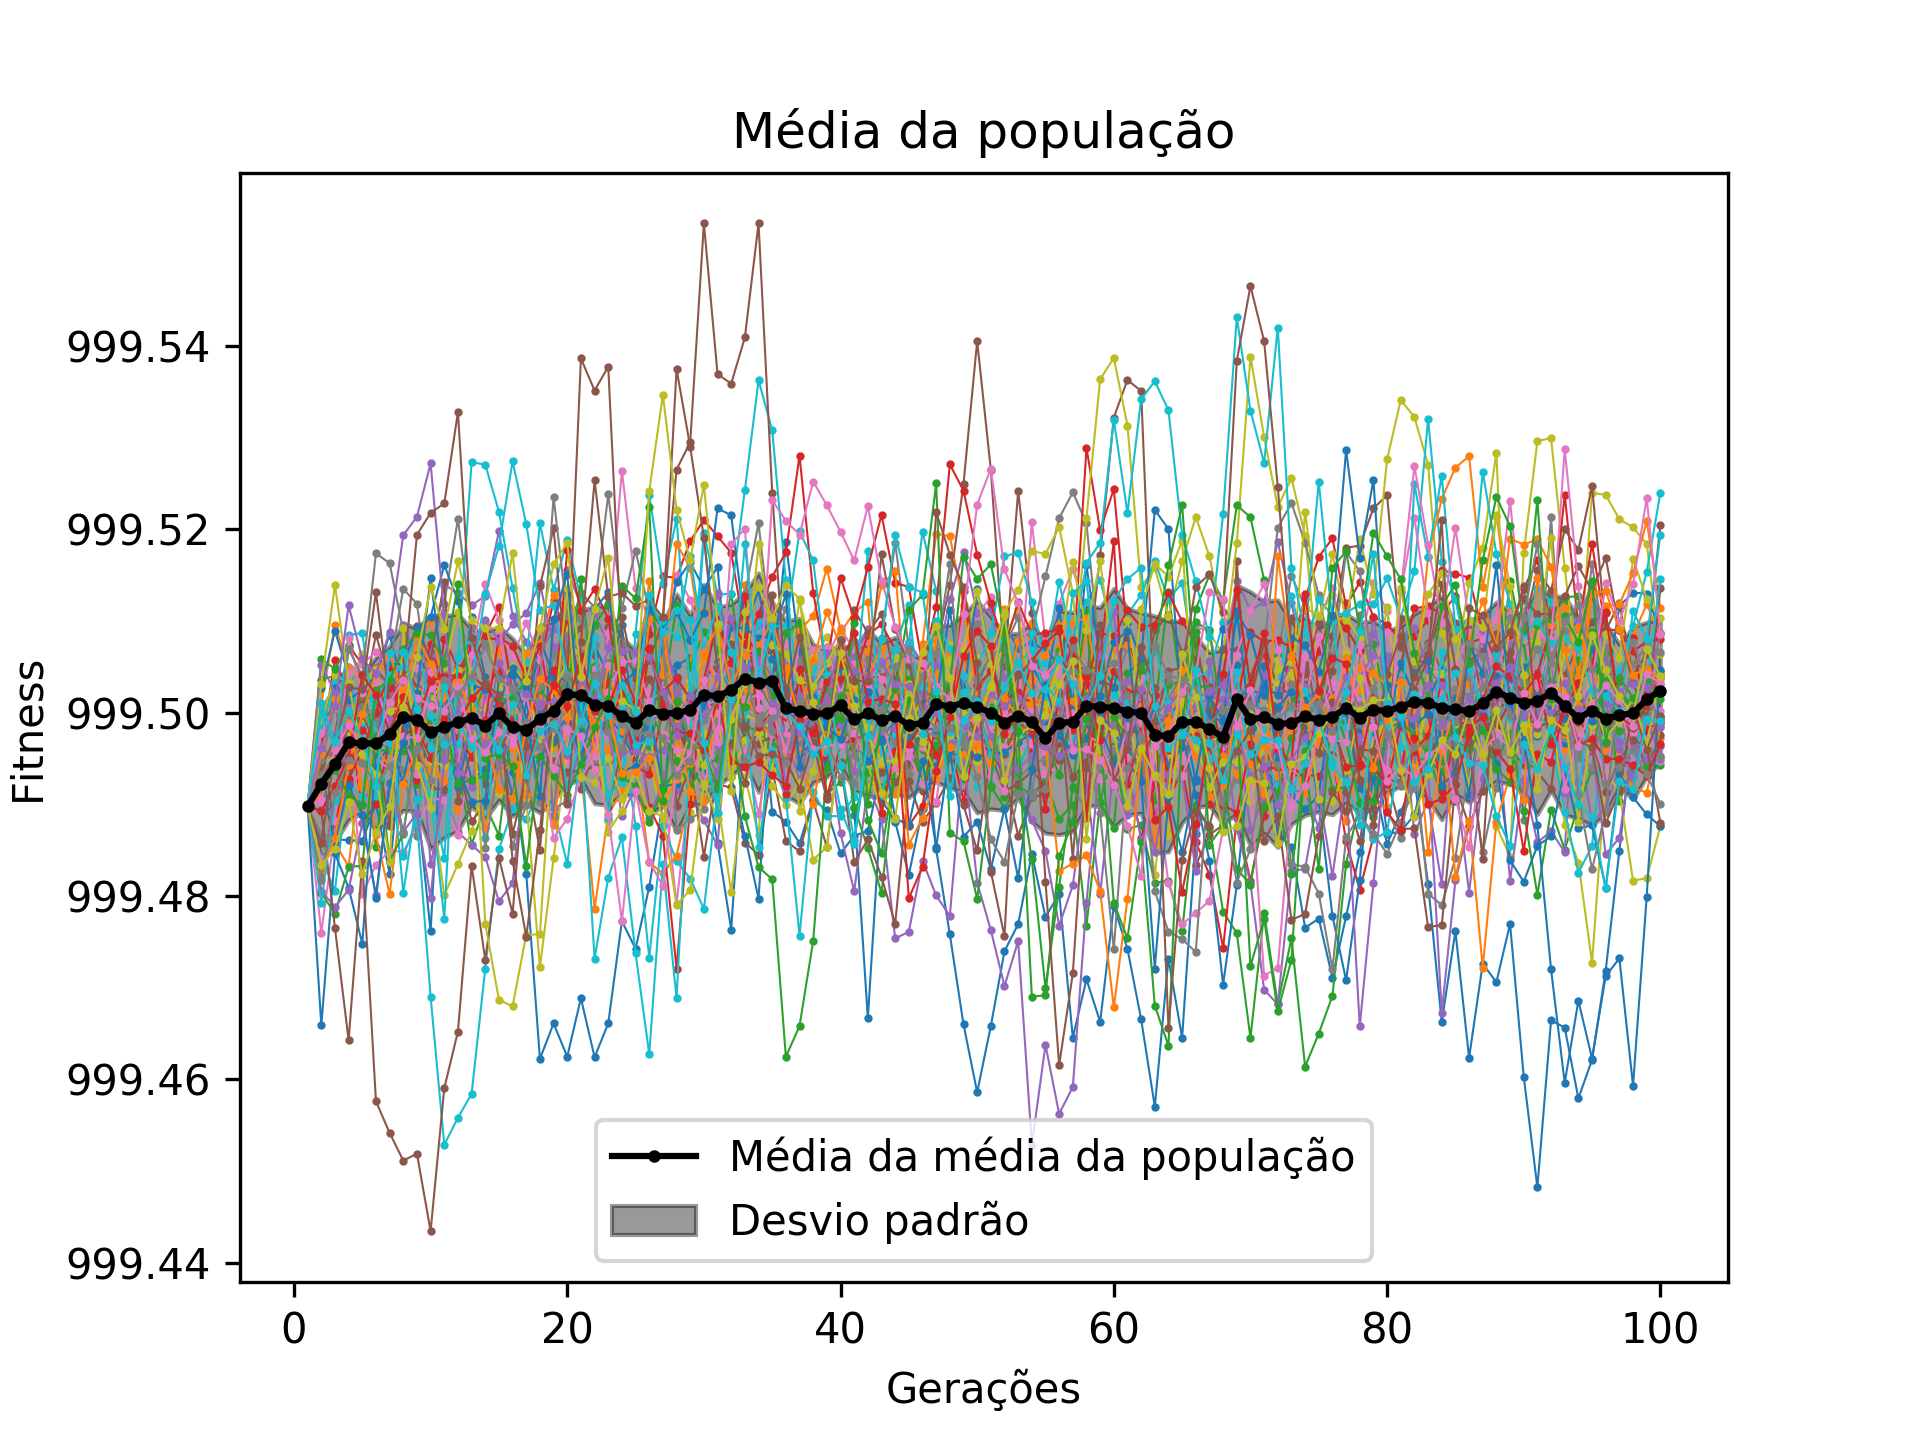
\includegraphics[width=1\textwidth]{./imgs/f6_prop/fitness_vs_gen_pop.png}
		\caption{Média da população de todos os experimentos ao longo das gerações.
		Em preto é mostrado o comportamento médio dos 50 experimentos.}
	\end{subfigure}
	\caption{Resultados obtidos no teste número 3 da tabela~\ref{tab:f6_prop}}
\end{figure}


	\begin{figure}[htb]
	\begin{subfigure}{.5\textwidth}
		\centering
		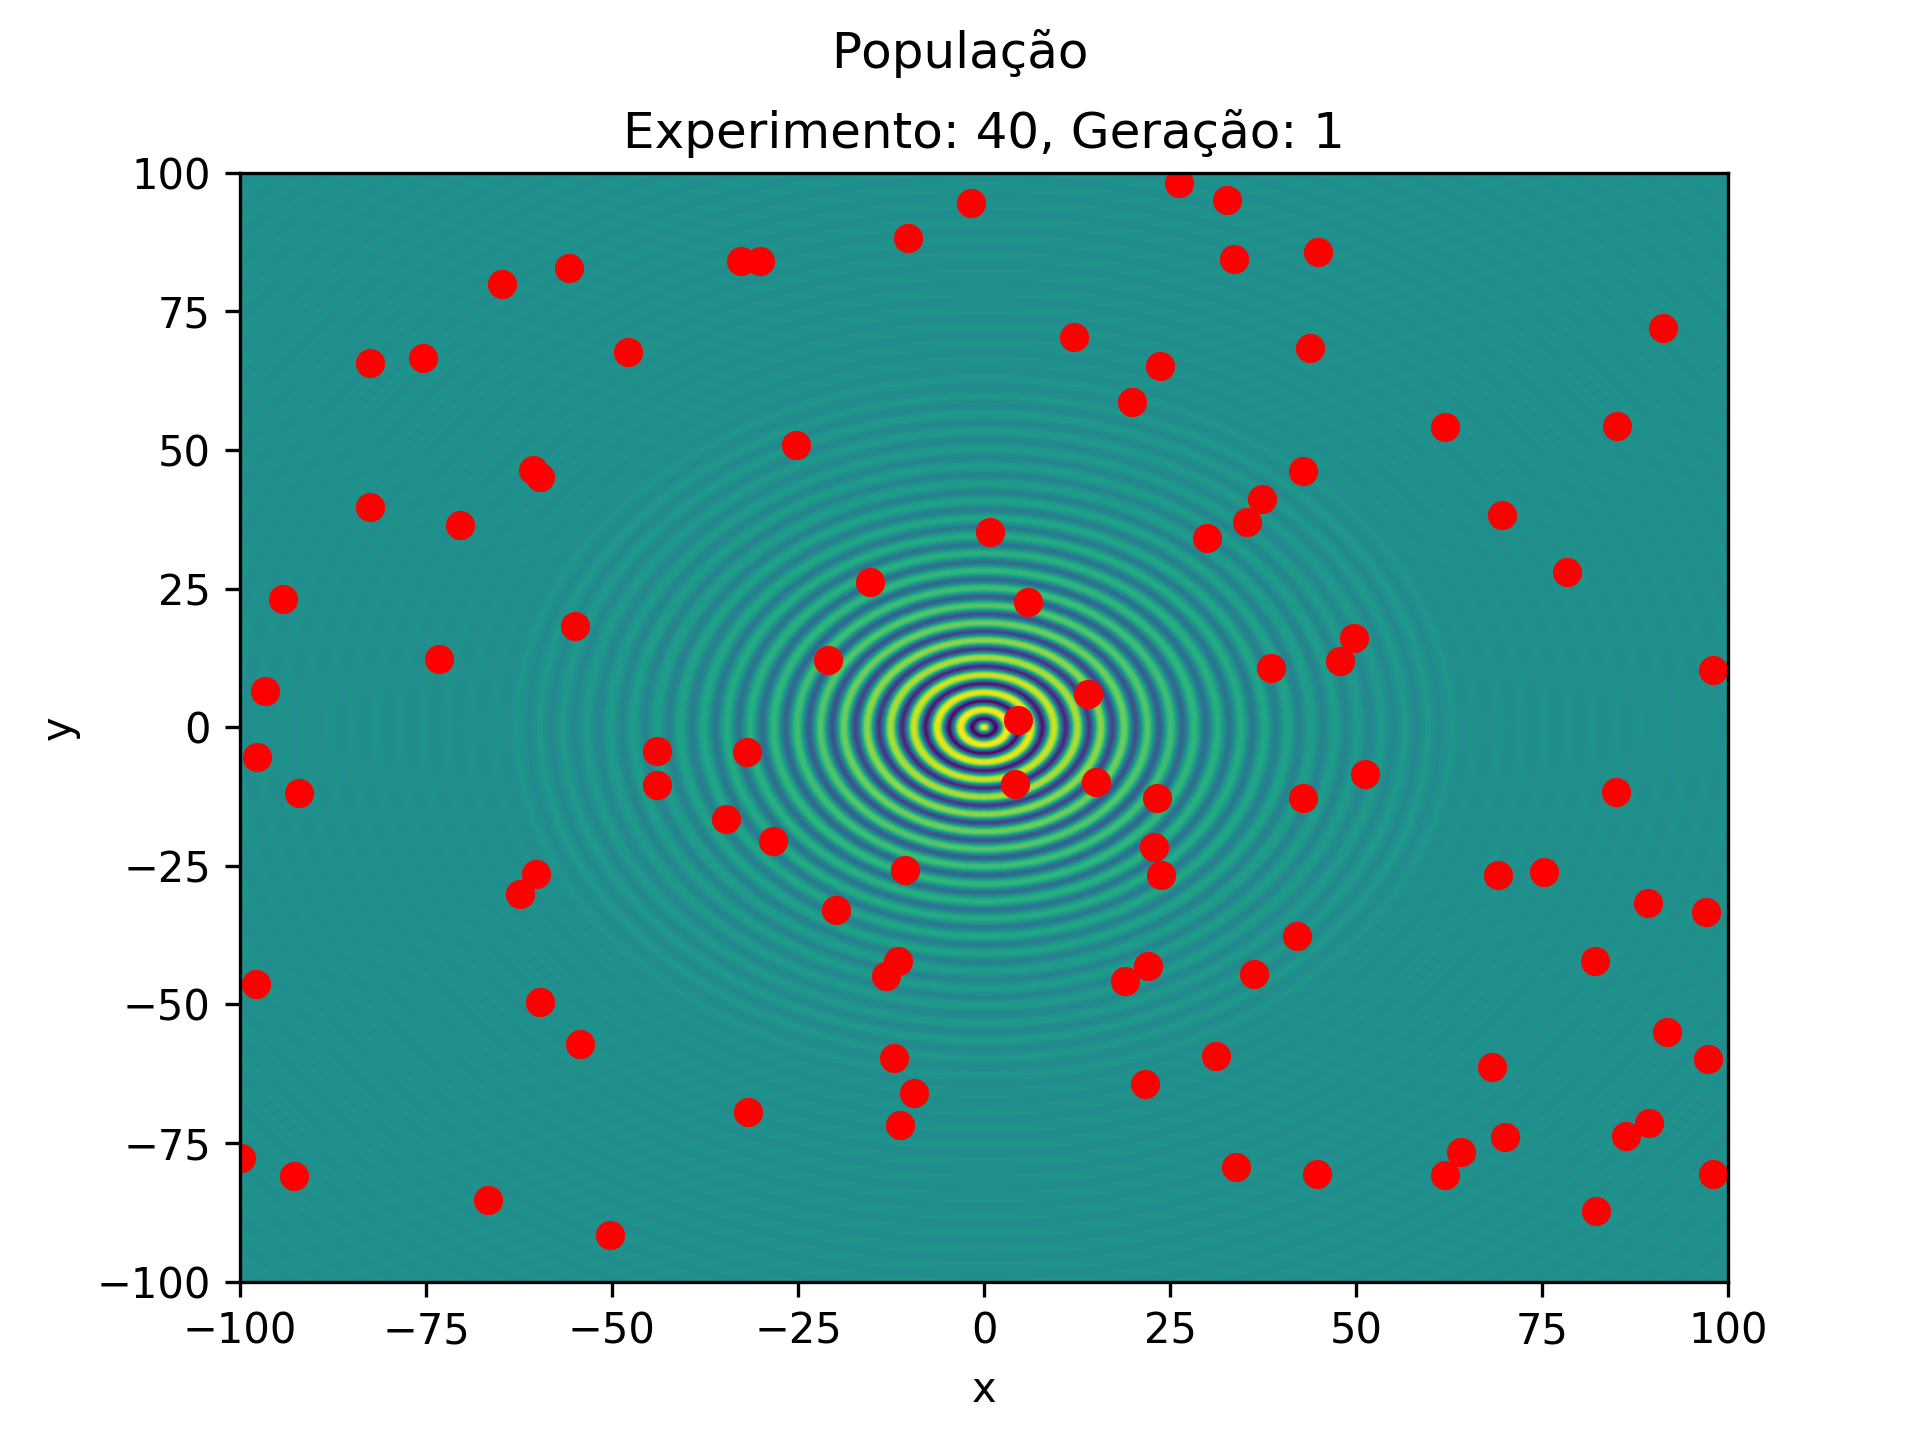
\includegraphics[width=0.9\linewidth]{./imgs/f6_prop/population_gen_1_exp_40.png}
	  \end{subfigure}
	  \begin{subfigure}{.5\textwidth}
		\centering
		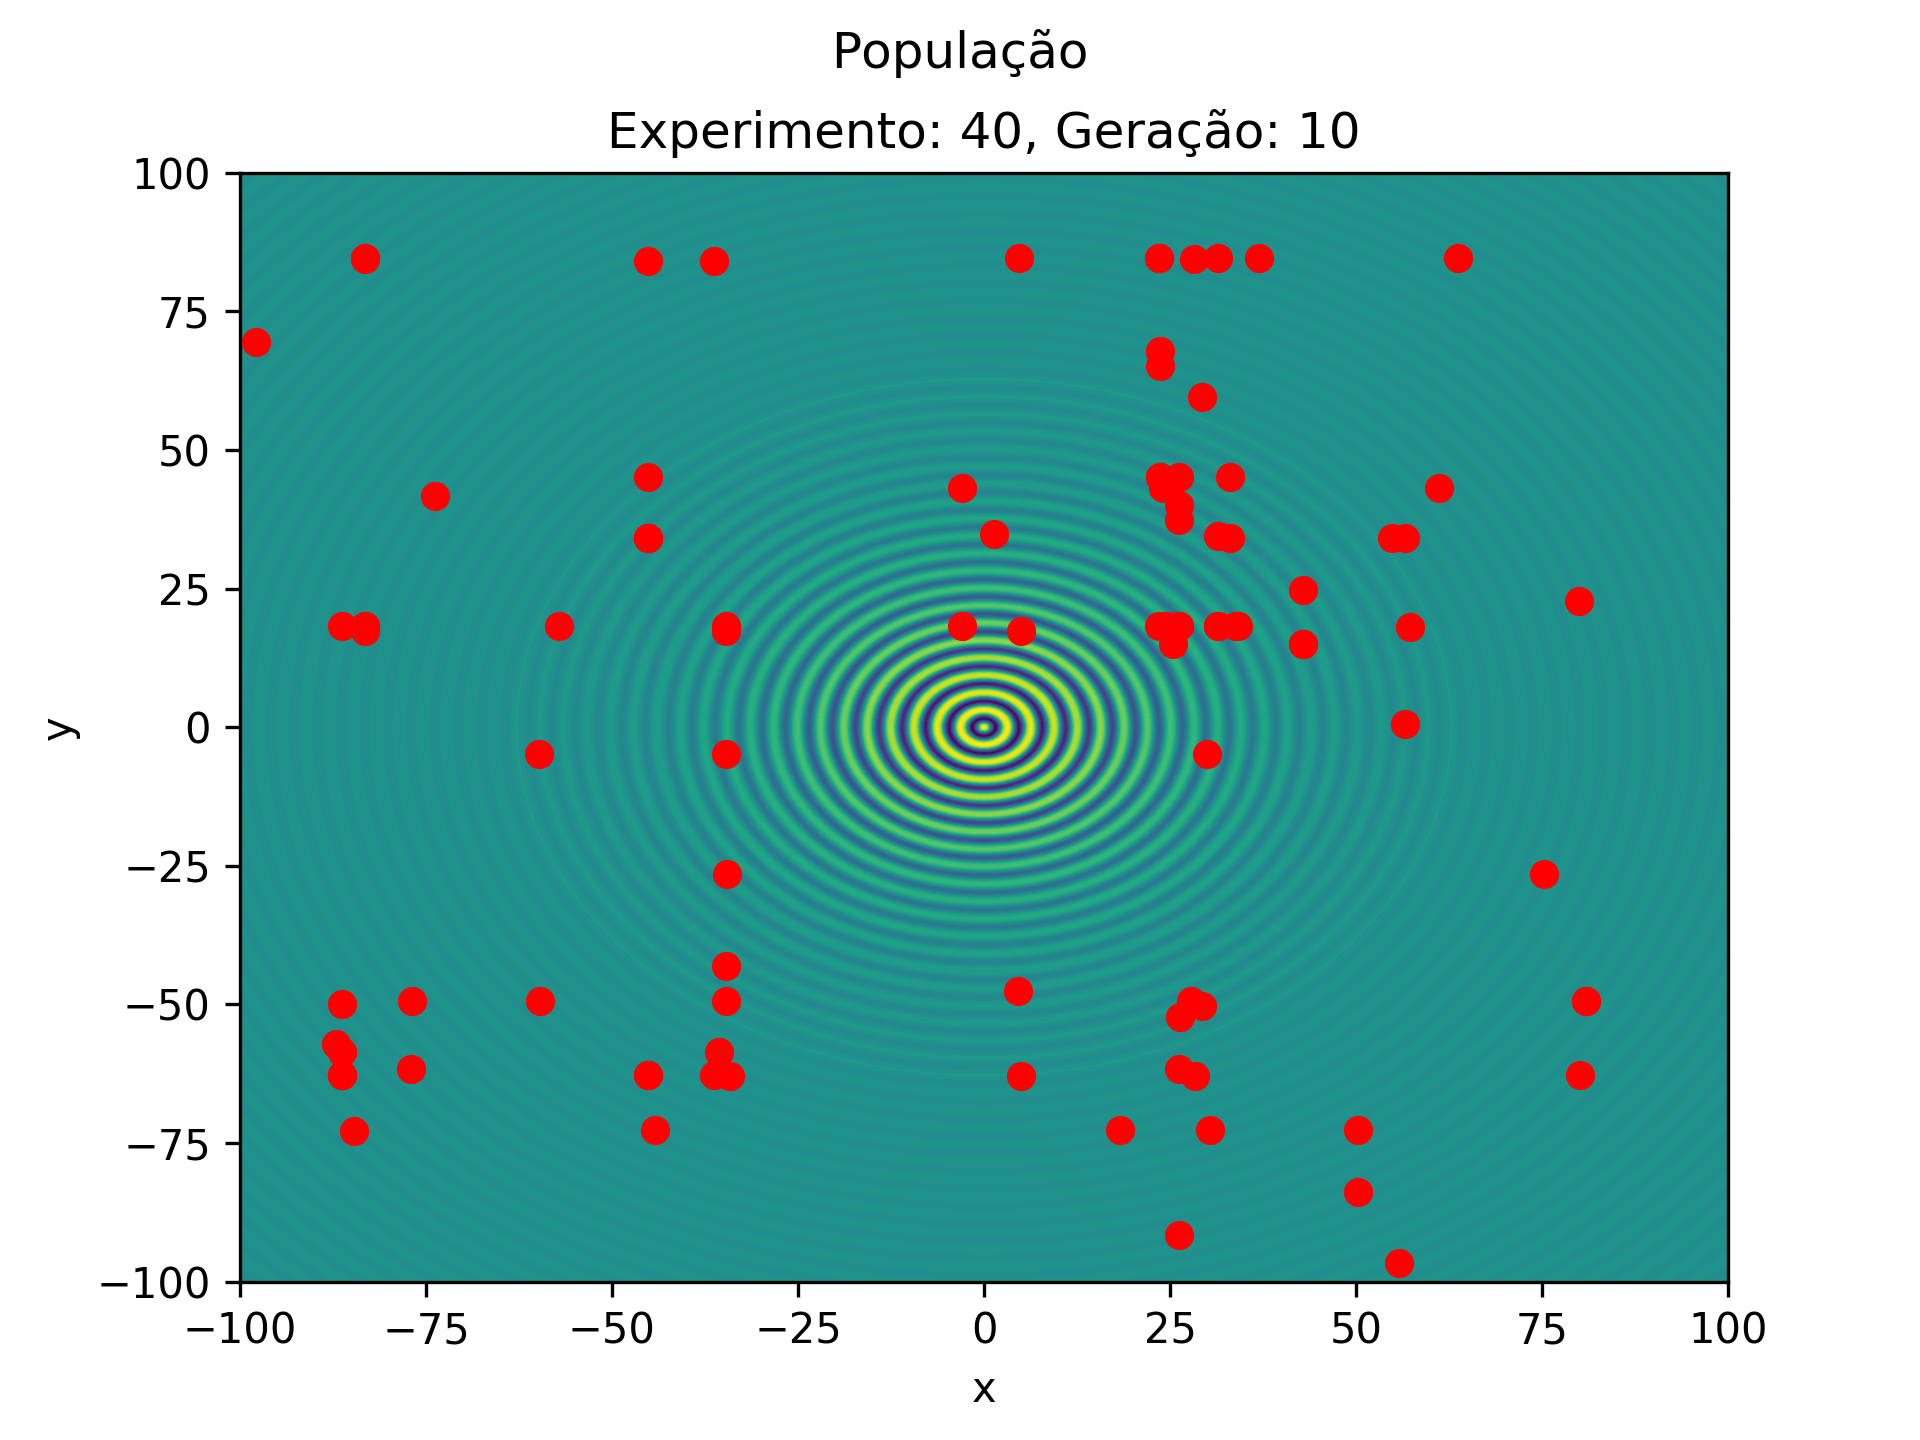
\includegraphics[width=0.9\linewidth]{./imgs/f6_prop/population_gen_10_exp_40.png}
	  \end{subfigure}
	  \begin{subfigure}{.5\textwidth}
		\centering
		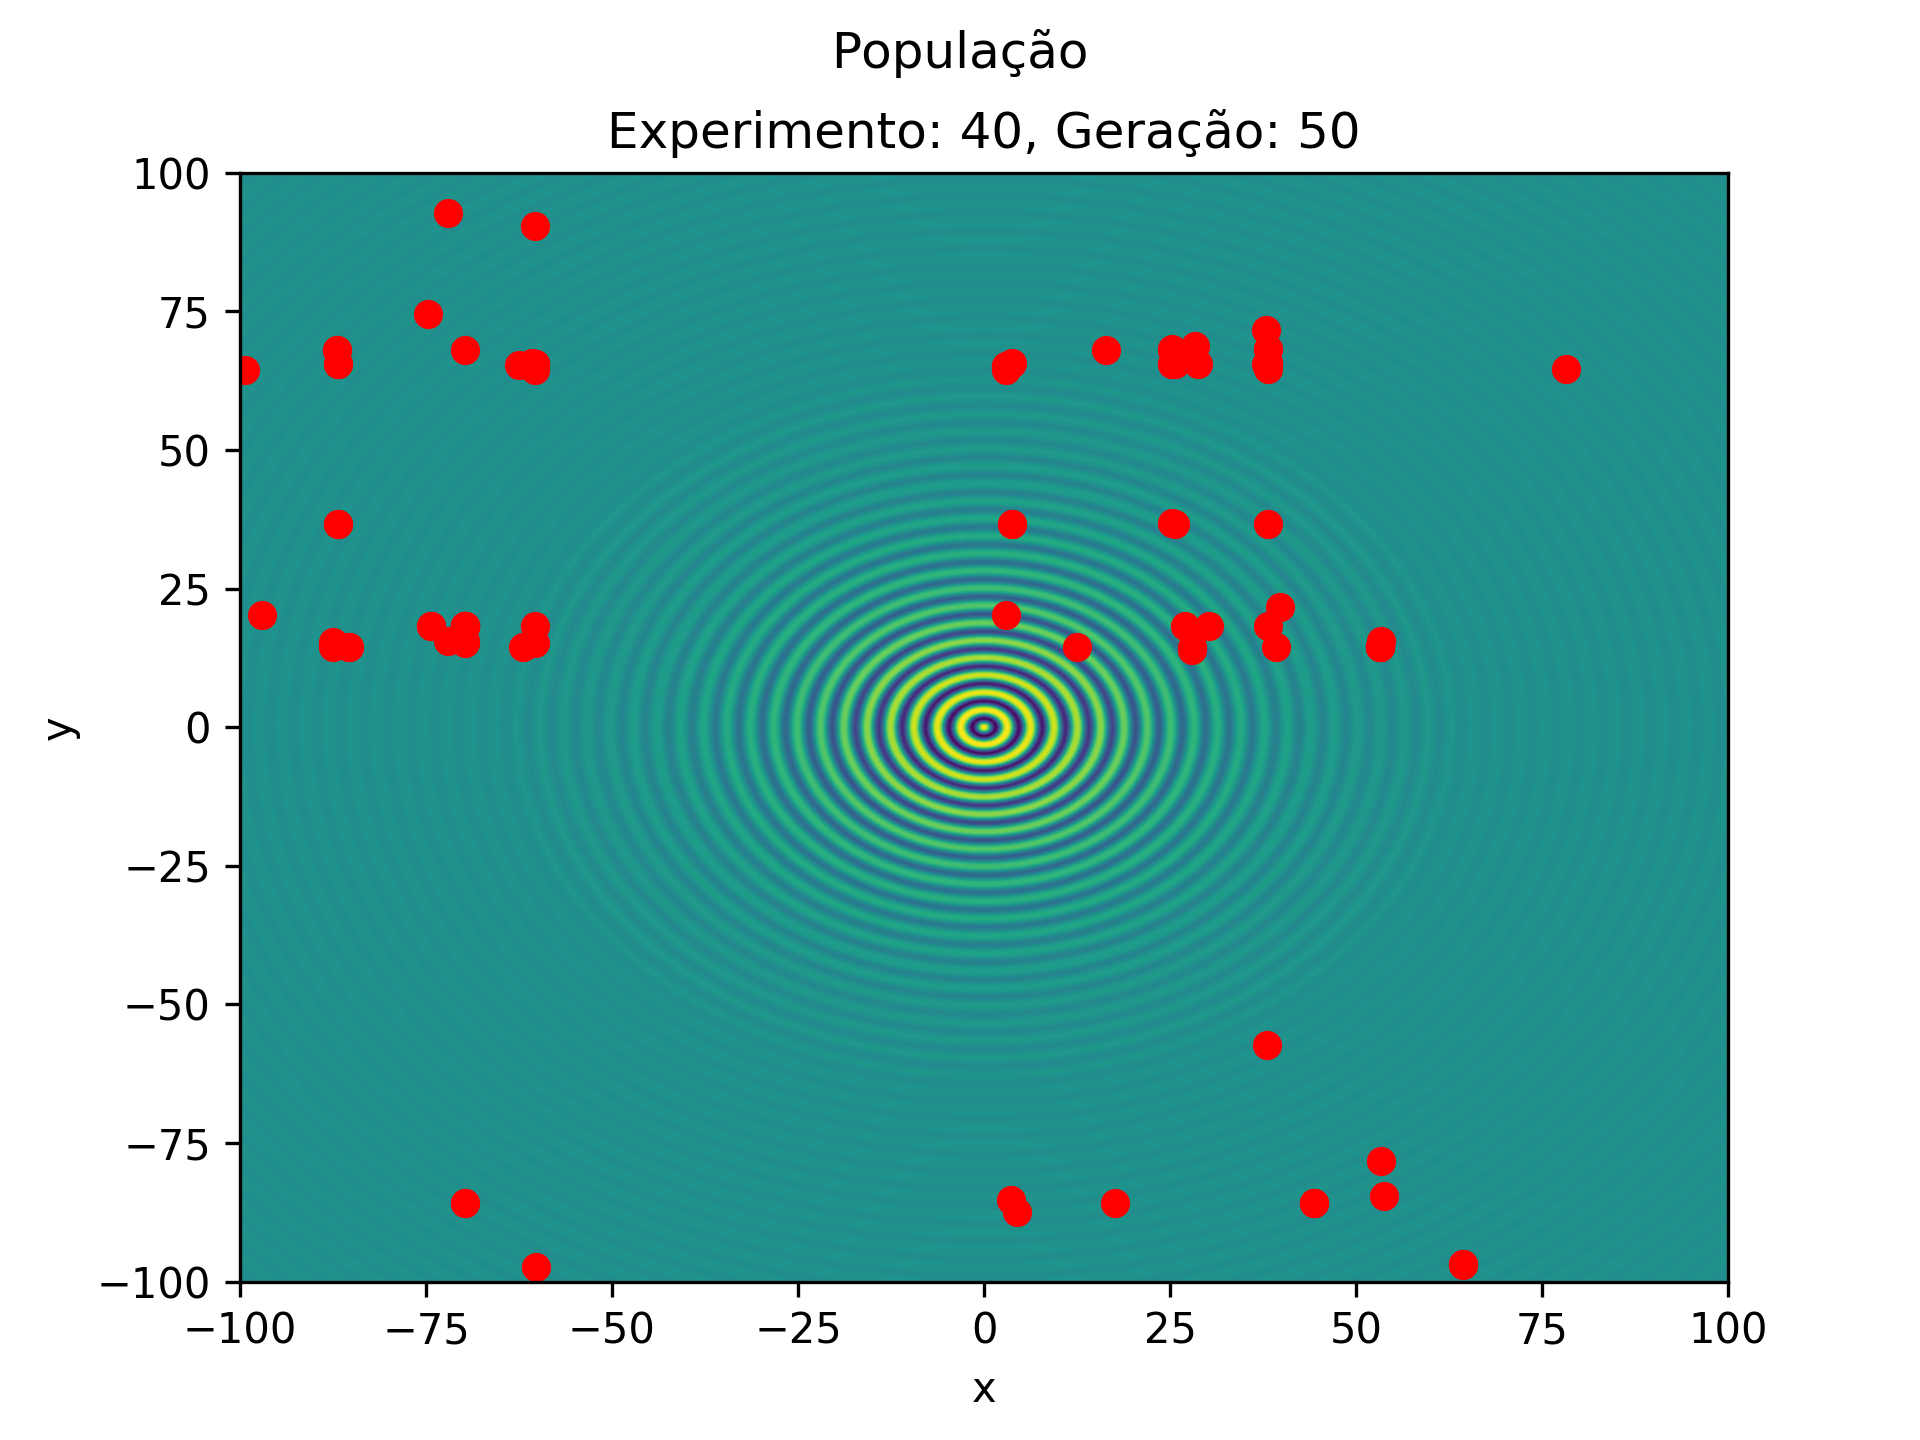
\includegraphics[width=0.9\linewidth]{./imgs/f6_prop/population_gen_50_exp_40.png}
	  \end{subfigure}
	  \begin{subfigure}{.5\textwidth}
		\centering
		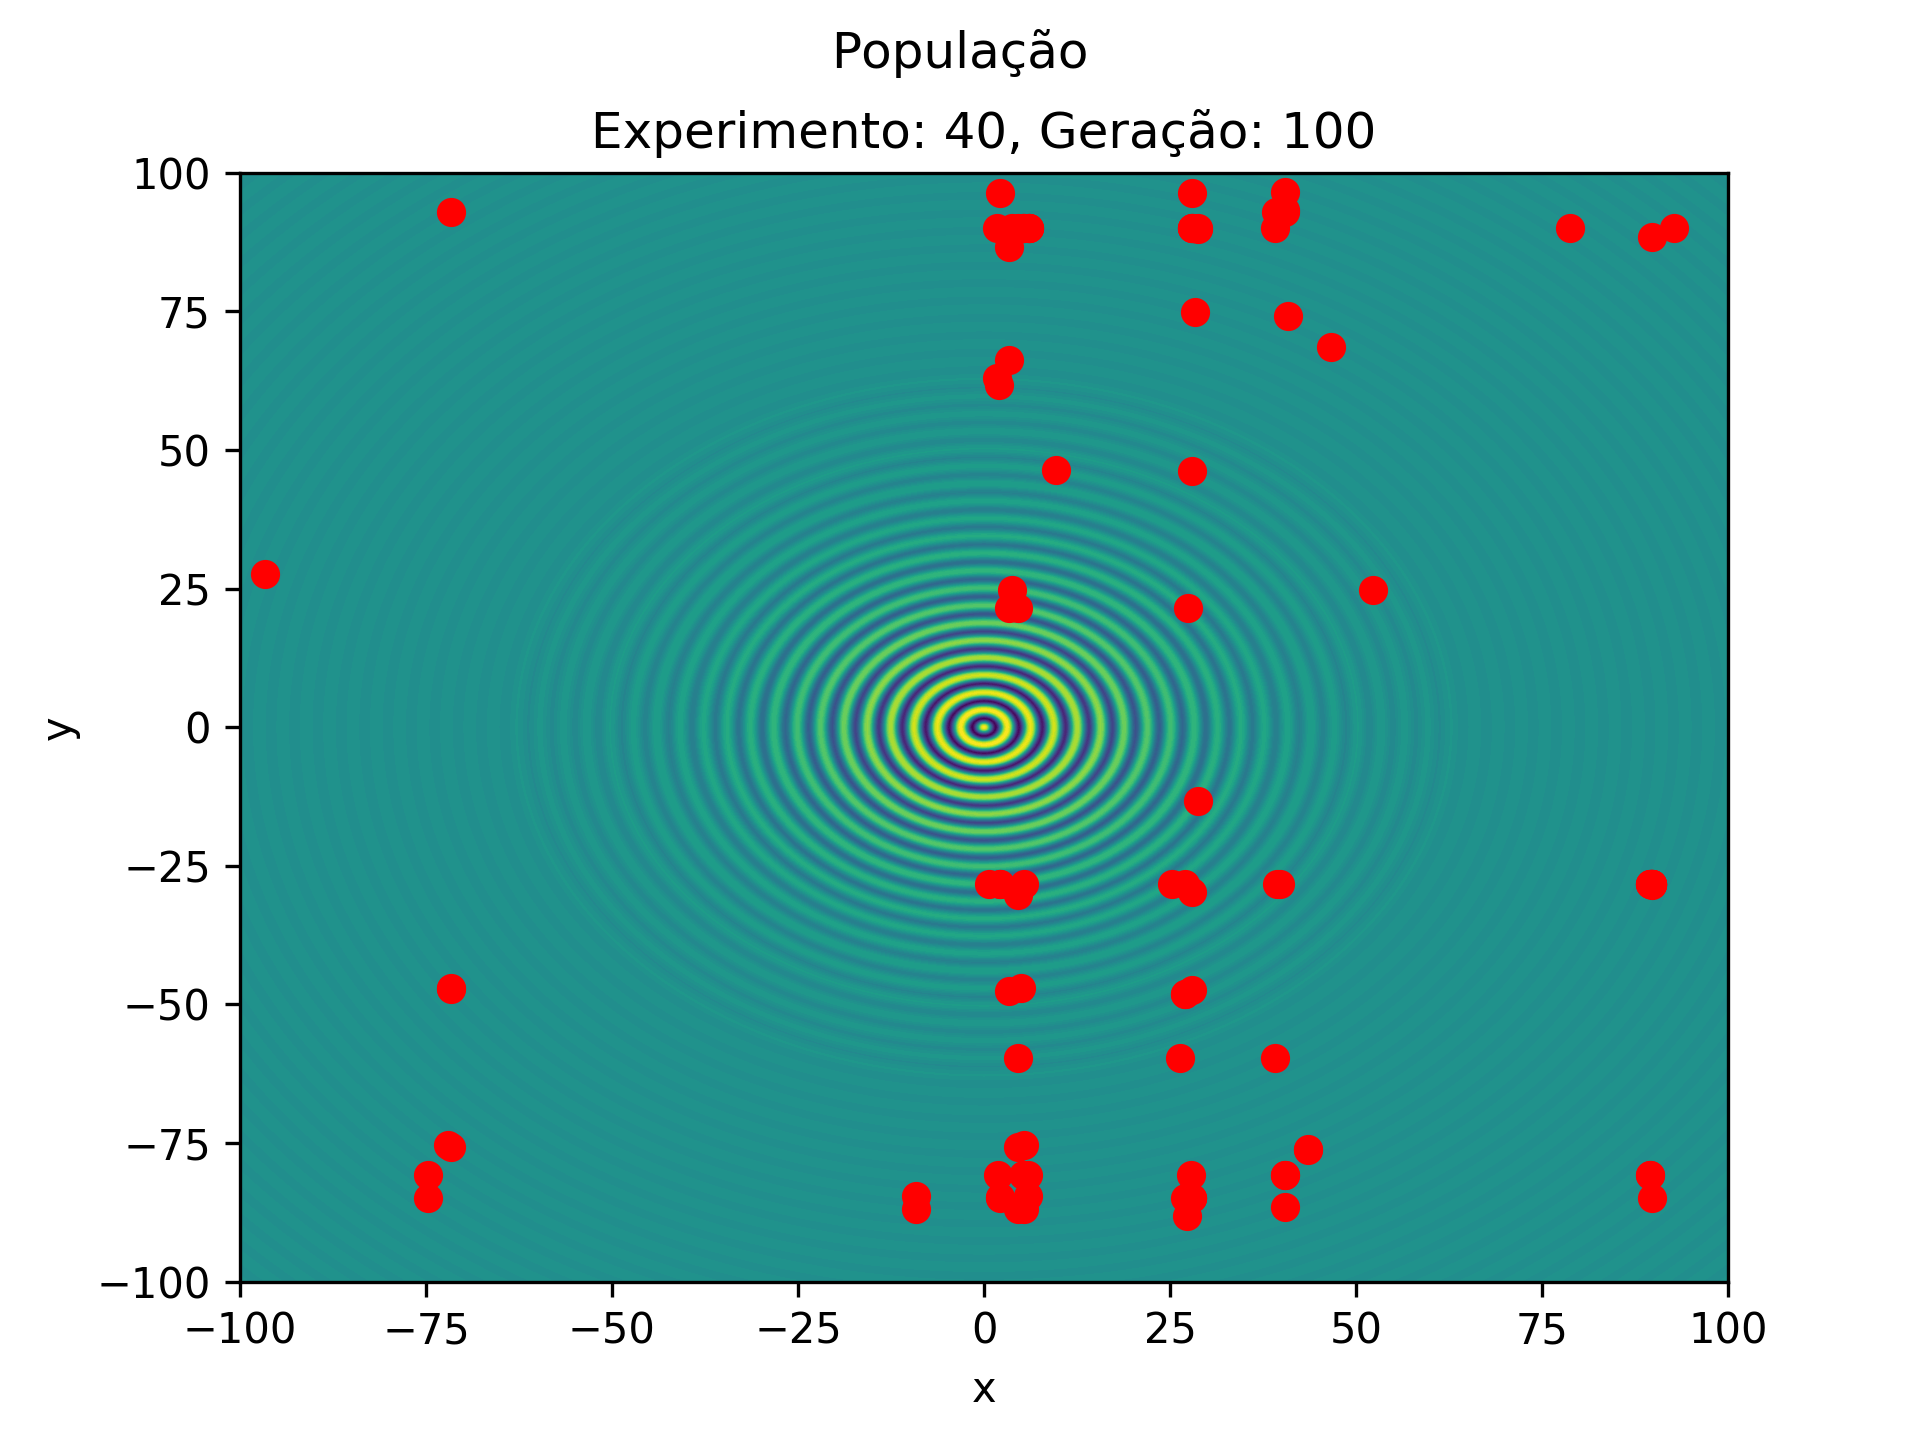
\includegraphics[width=0.9\linewidth]{./imgs/f6_prop/population_gen_100_exp_40.png}
	  \end{subfigure}
	\caption{Populações do experimento 40 nas gerações 1, 10, 50 e 100 para o teste número 3.}
	\end{figure}

	Posteriormente, utilizando a normalização linear obtiveram-se resultados positivos para a função f6 elevada.
	Note que as escolhas do valor máximo e mínimo para fazer a normalização definem a presão seletiva do algoritimo
	se seleção. Assim, foram realizados teste com diferentes valores de $max$ e $min$.

	\begin{table}[htb]
		\centering
		\begin{tabular}{|c|c|c|}
			\hline
			\rowcolor[HTML]{9B9B9B}
			Teste & Média do melhor indíviduo & Média da população \\\hline
			1 & 999.97301 & 999.84923 \\\hline
			2 & 999.95522 & 999.81788 \\\hline
			3 & 999.94695 & 999.81014 \\\hline
			4 & 999.96168 & 999.82242 \\\hline
			5 & 999.95617 & 999.81577 \\\hline
			Média Final & 999.95860 & 999.82309 \\\hline
		\end{tabular}
		\caption{Resultados da função f6 elevada utilizando seleção
		proporcional ao fitness com normalização linear, $min = 0$ e $max = 1$. \label{tab:f6_norm_01}}
	\end{table}

	\begin{figure}[htb]
		\begin{subfigure}{.45\textwidth}
			\centering
			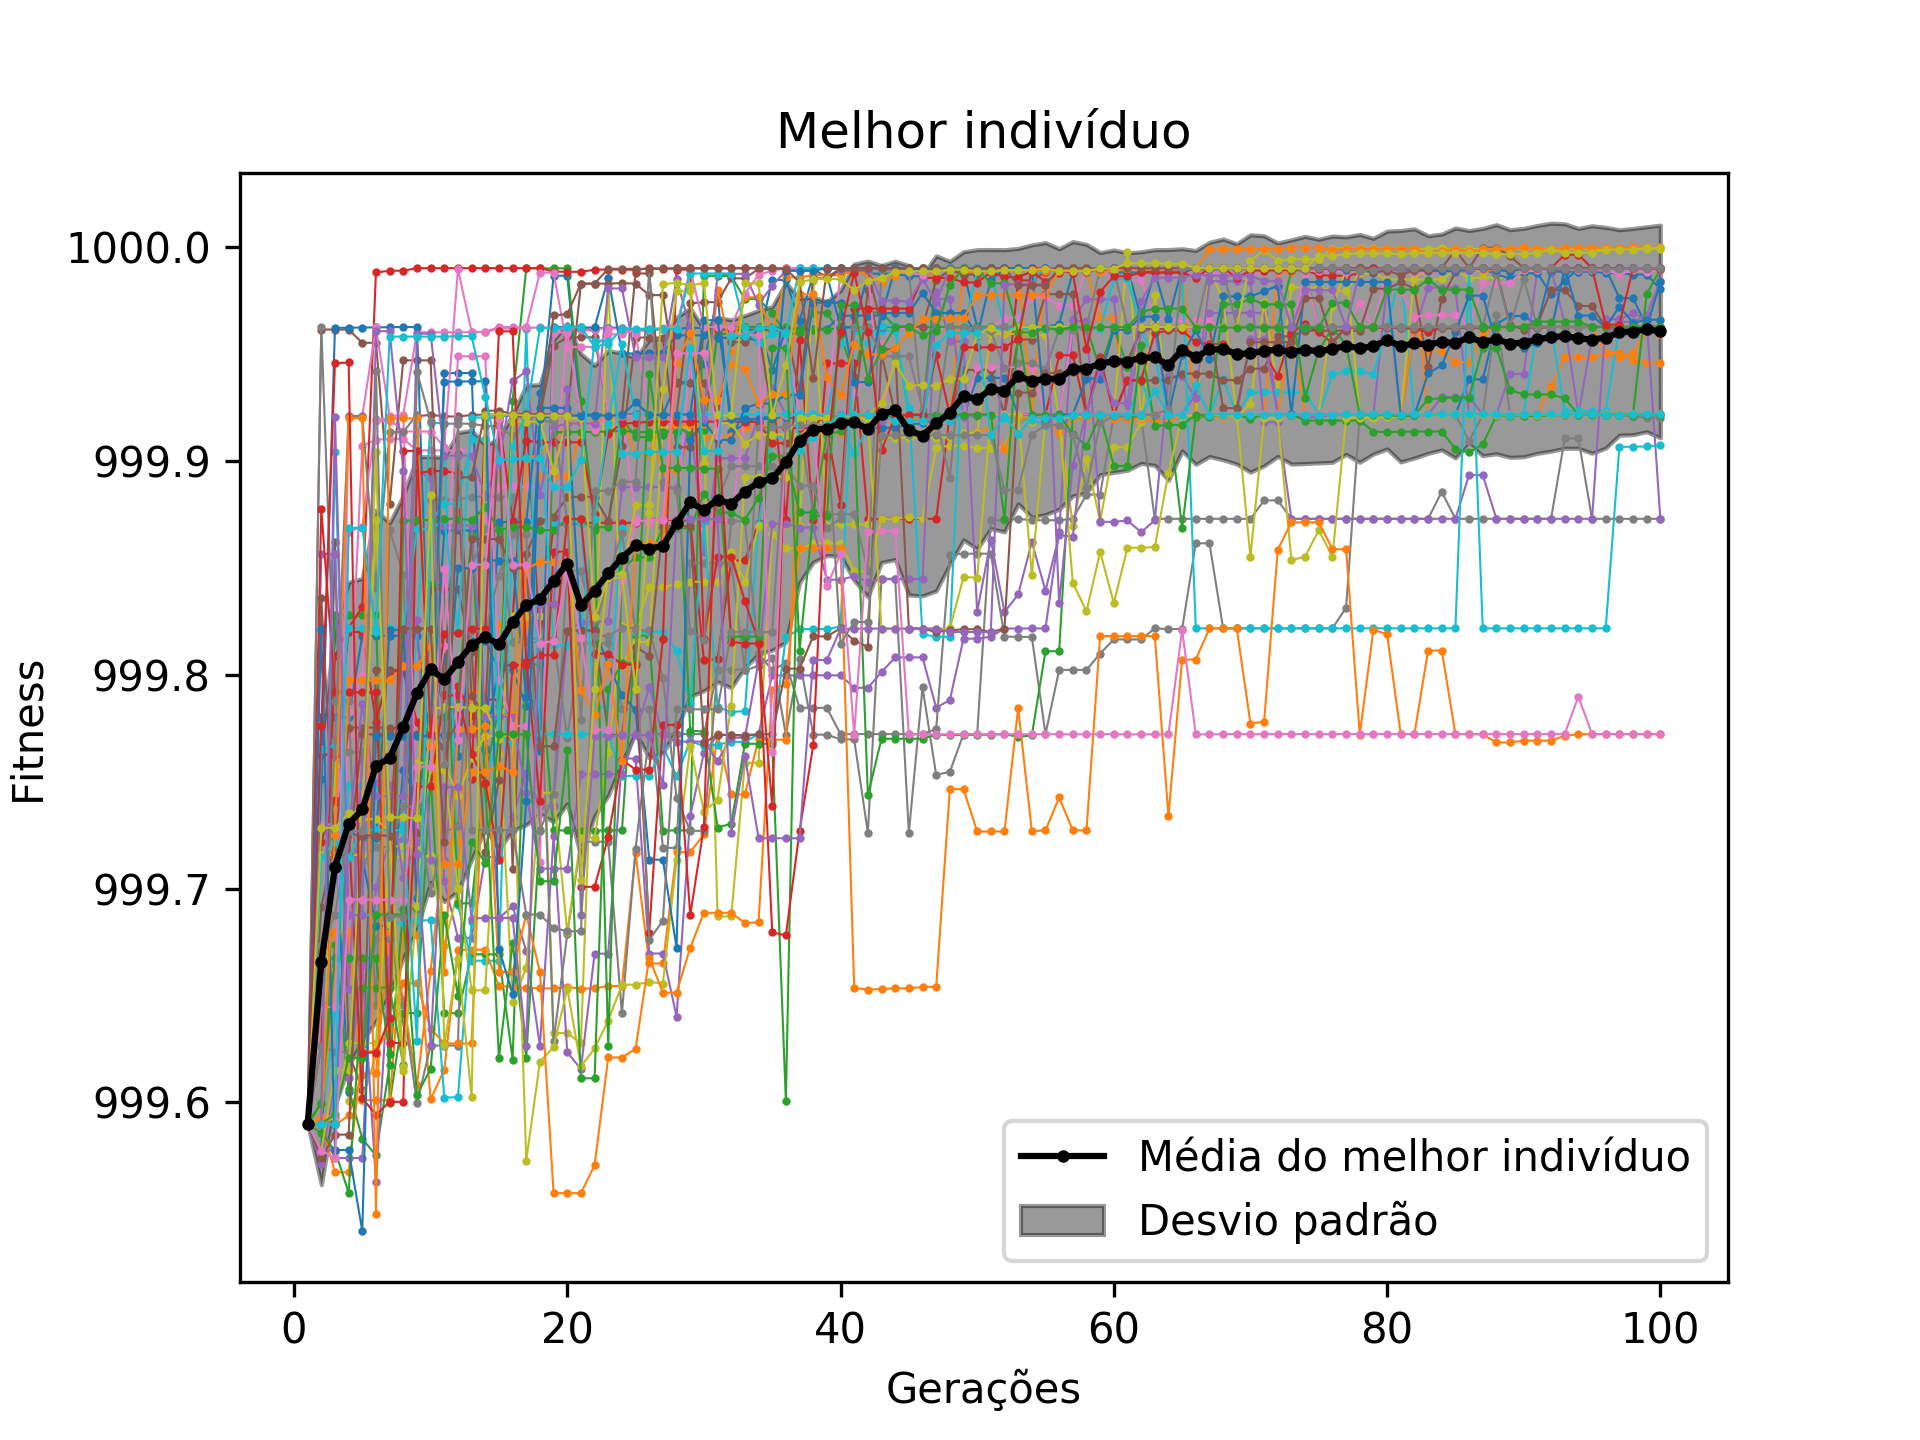
\includegraphics[width=1\textwidth]{./imgs/f6_norm_01/fitness_vs_gen_best.png}
			\caption{Melhores indíviduos de todos os experimentos ao longo das gerações.
			Em preto é mostrado o comportamento médio dos 50 experimentos. }
		\end{subfigure}
		\hfill
		\begin{subfigure}{.45\textwidth}
			\centering
			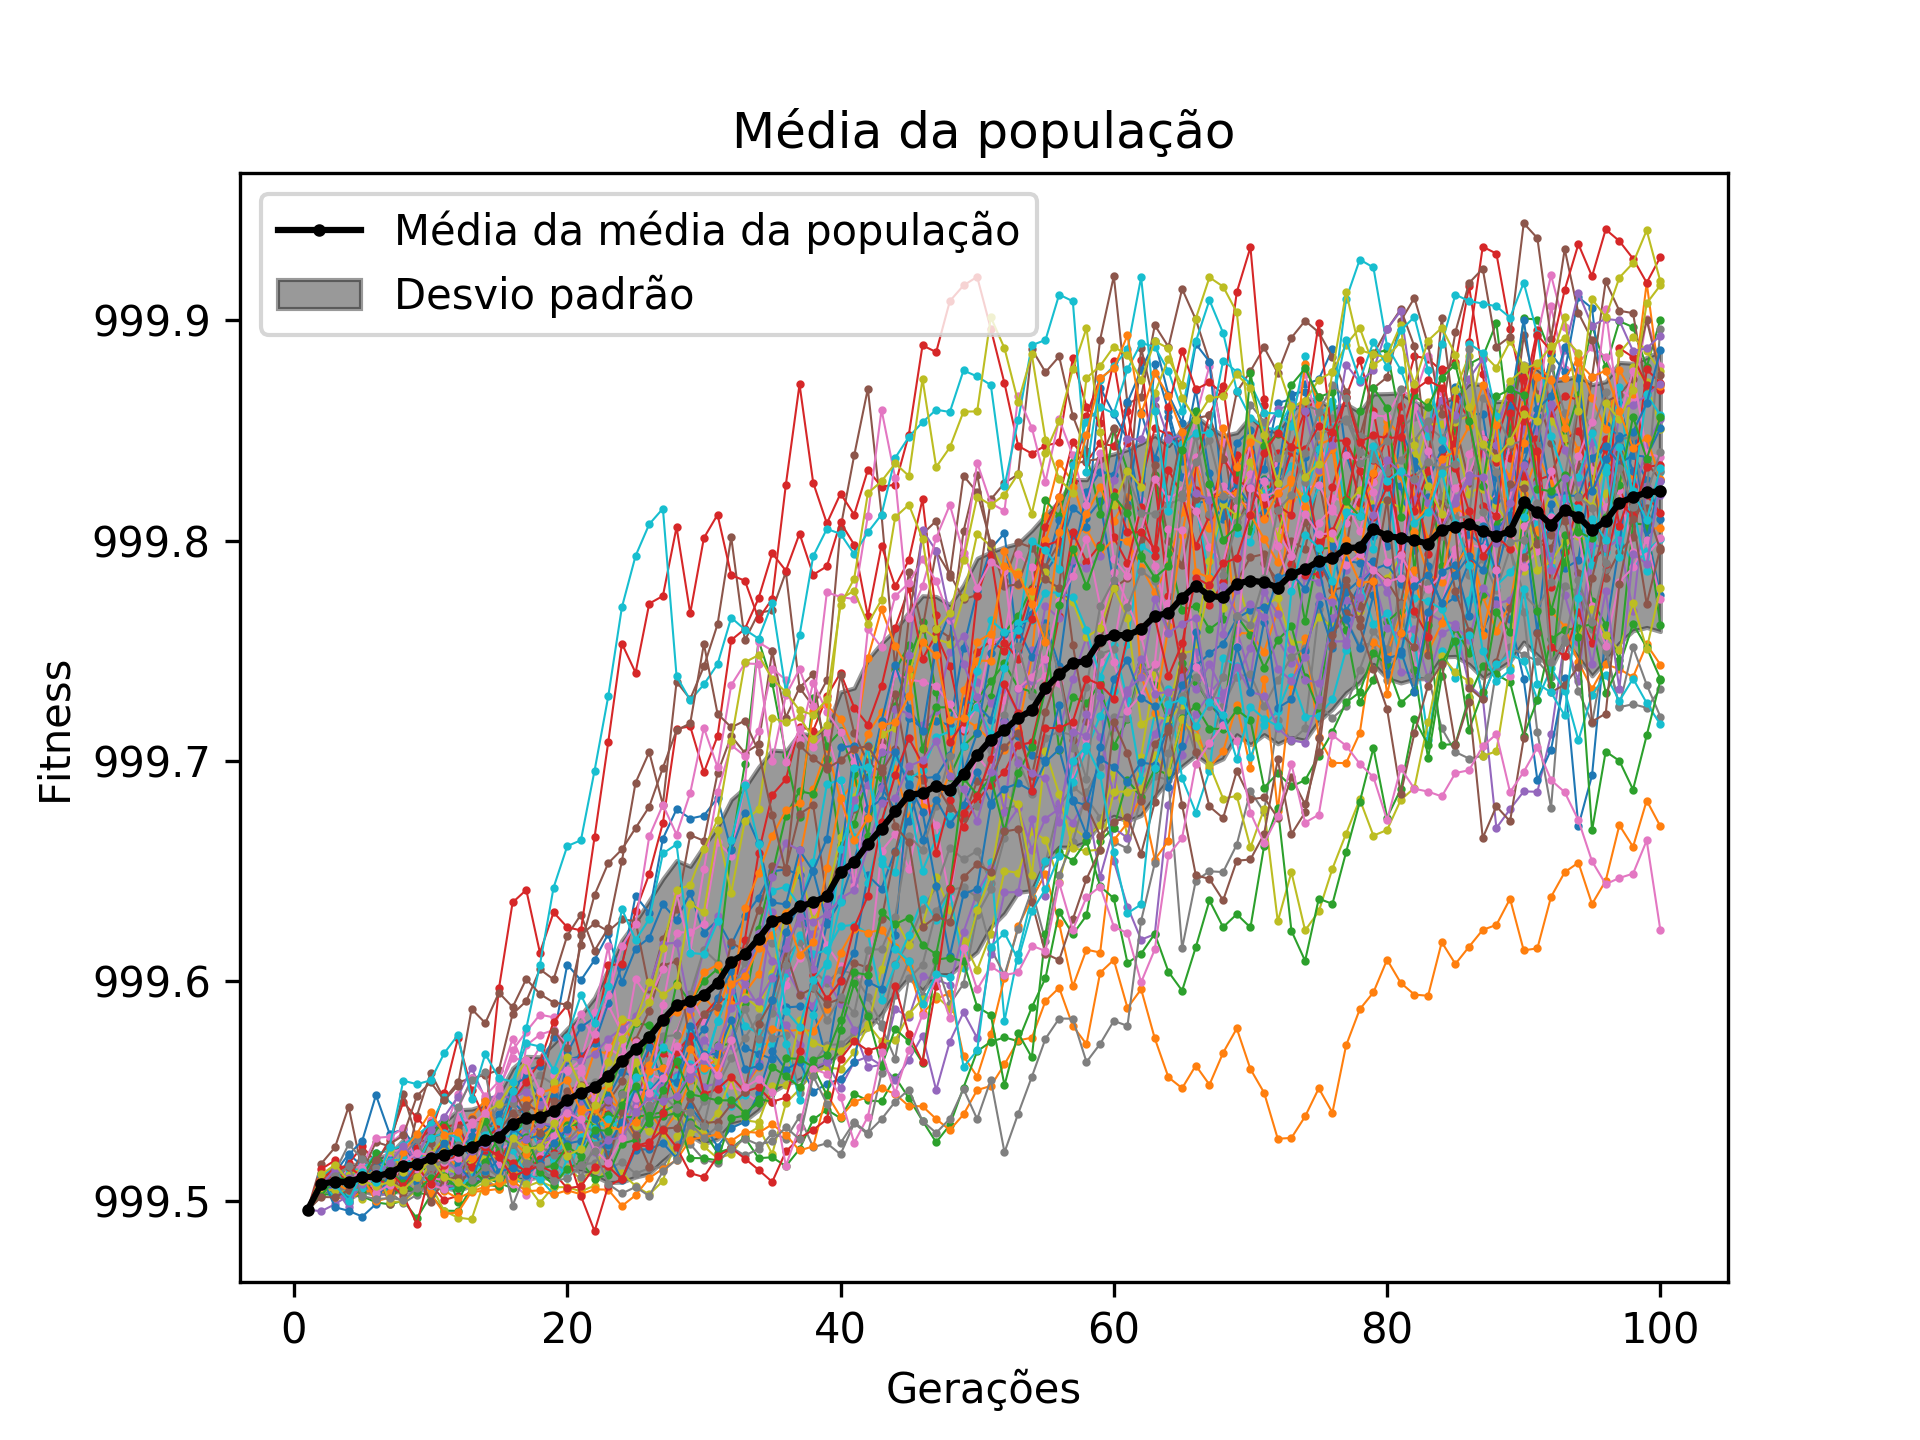
\includegraphics[width=1\textwidth]{./imgs/f6_norm_01/fitness_vs_gen_pop.png}
			\caption{Média da população de todos os experimentos ao longo das gerações.
			Em preto é mostrado o comportamento médio dos 50 experimentos.}
		\end{subfigure}
		\caption{Resultados obtidos no teste número 4 da tabela~\ref{tab:f6_norm_01}}
	\end{figure}

	A tabela~\ref{tab:f6_norm_01} apresenta os resultados para o caso de $min = 0$ e $max = 1$.

		\begin{figure}[htb]
		\begin{subfigure}{.5\textwidth}
			\centering
			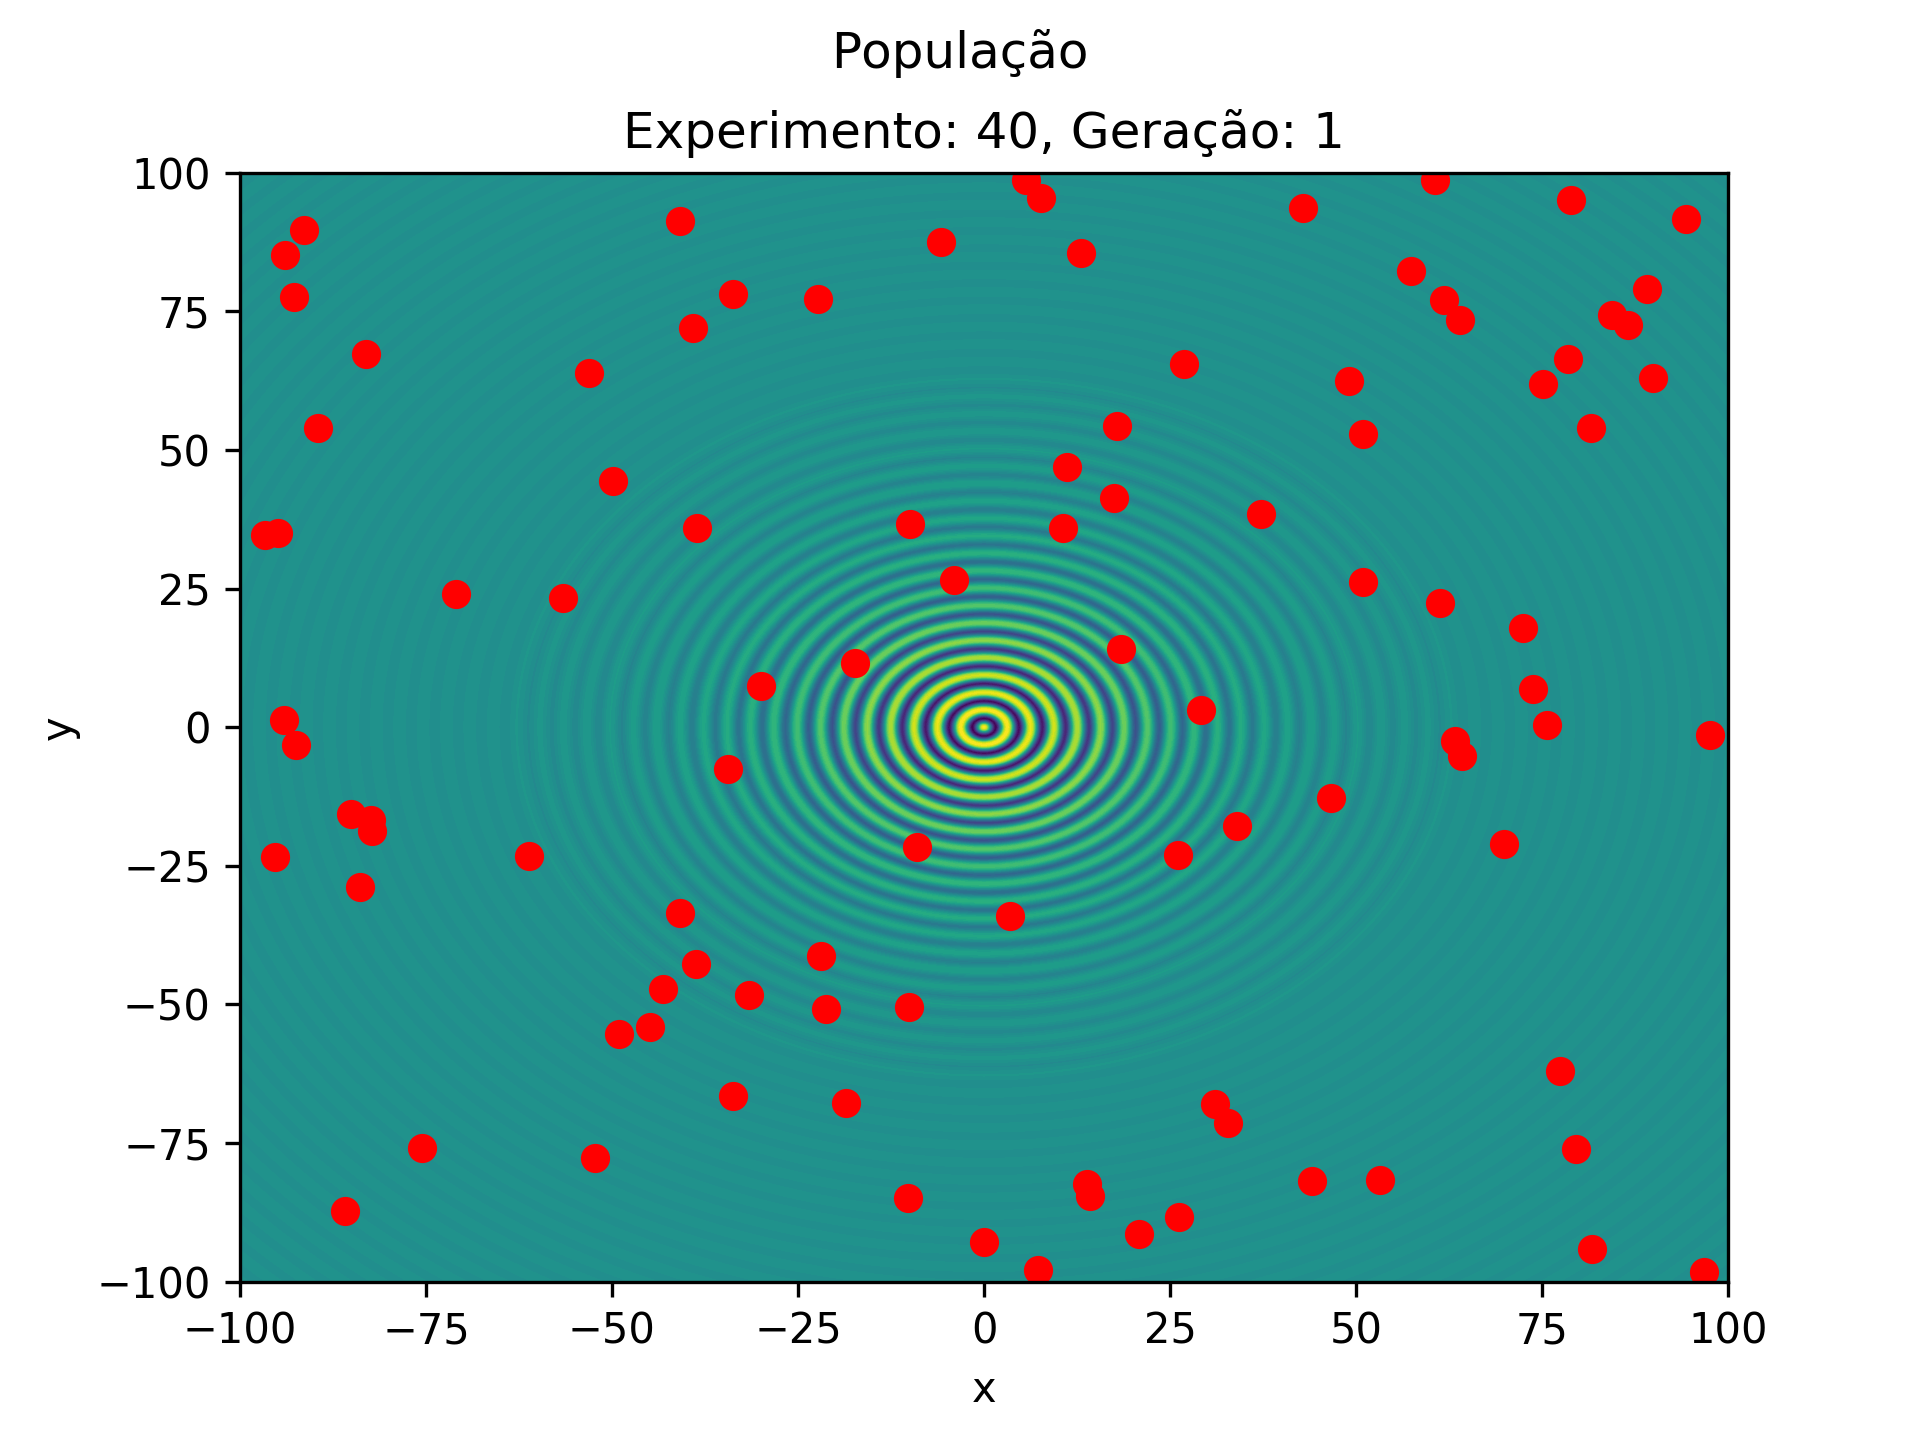
\includegraphics[width=0.9\linewidth]{./imgs/f6_norm_01/population_gen_1_exp_40.png}
		  \end{subfigure}
		  \begin{subfigure}{.5\textwidth}
			\centering
			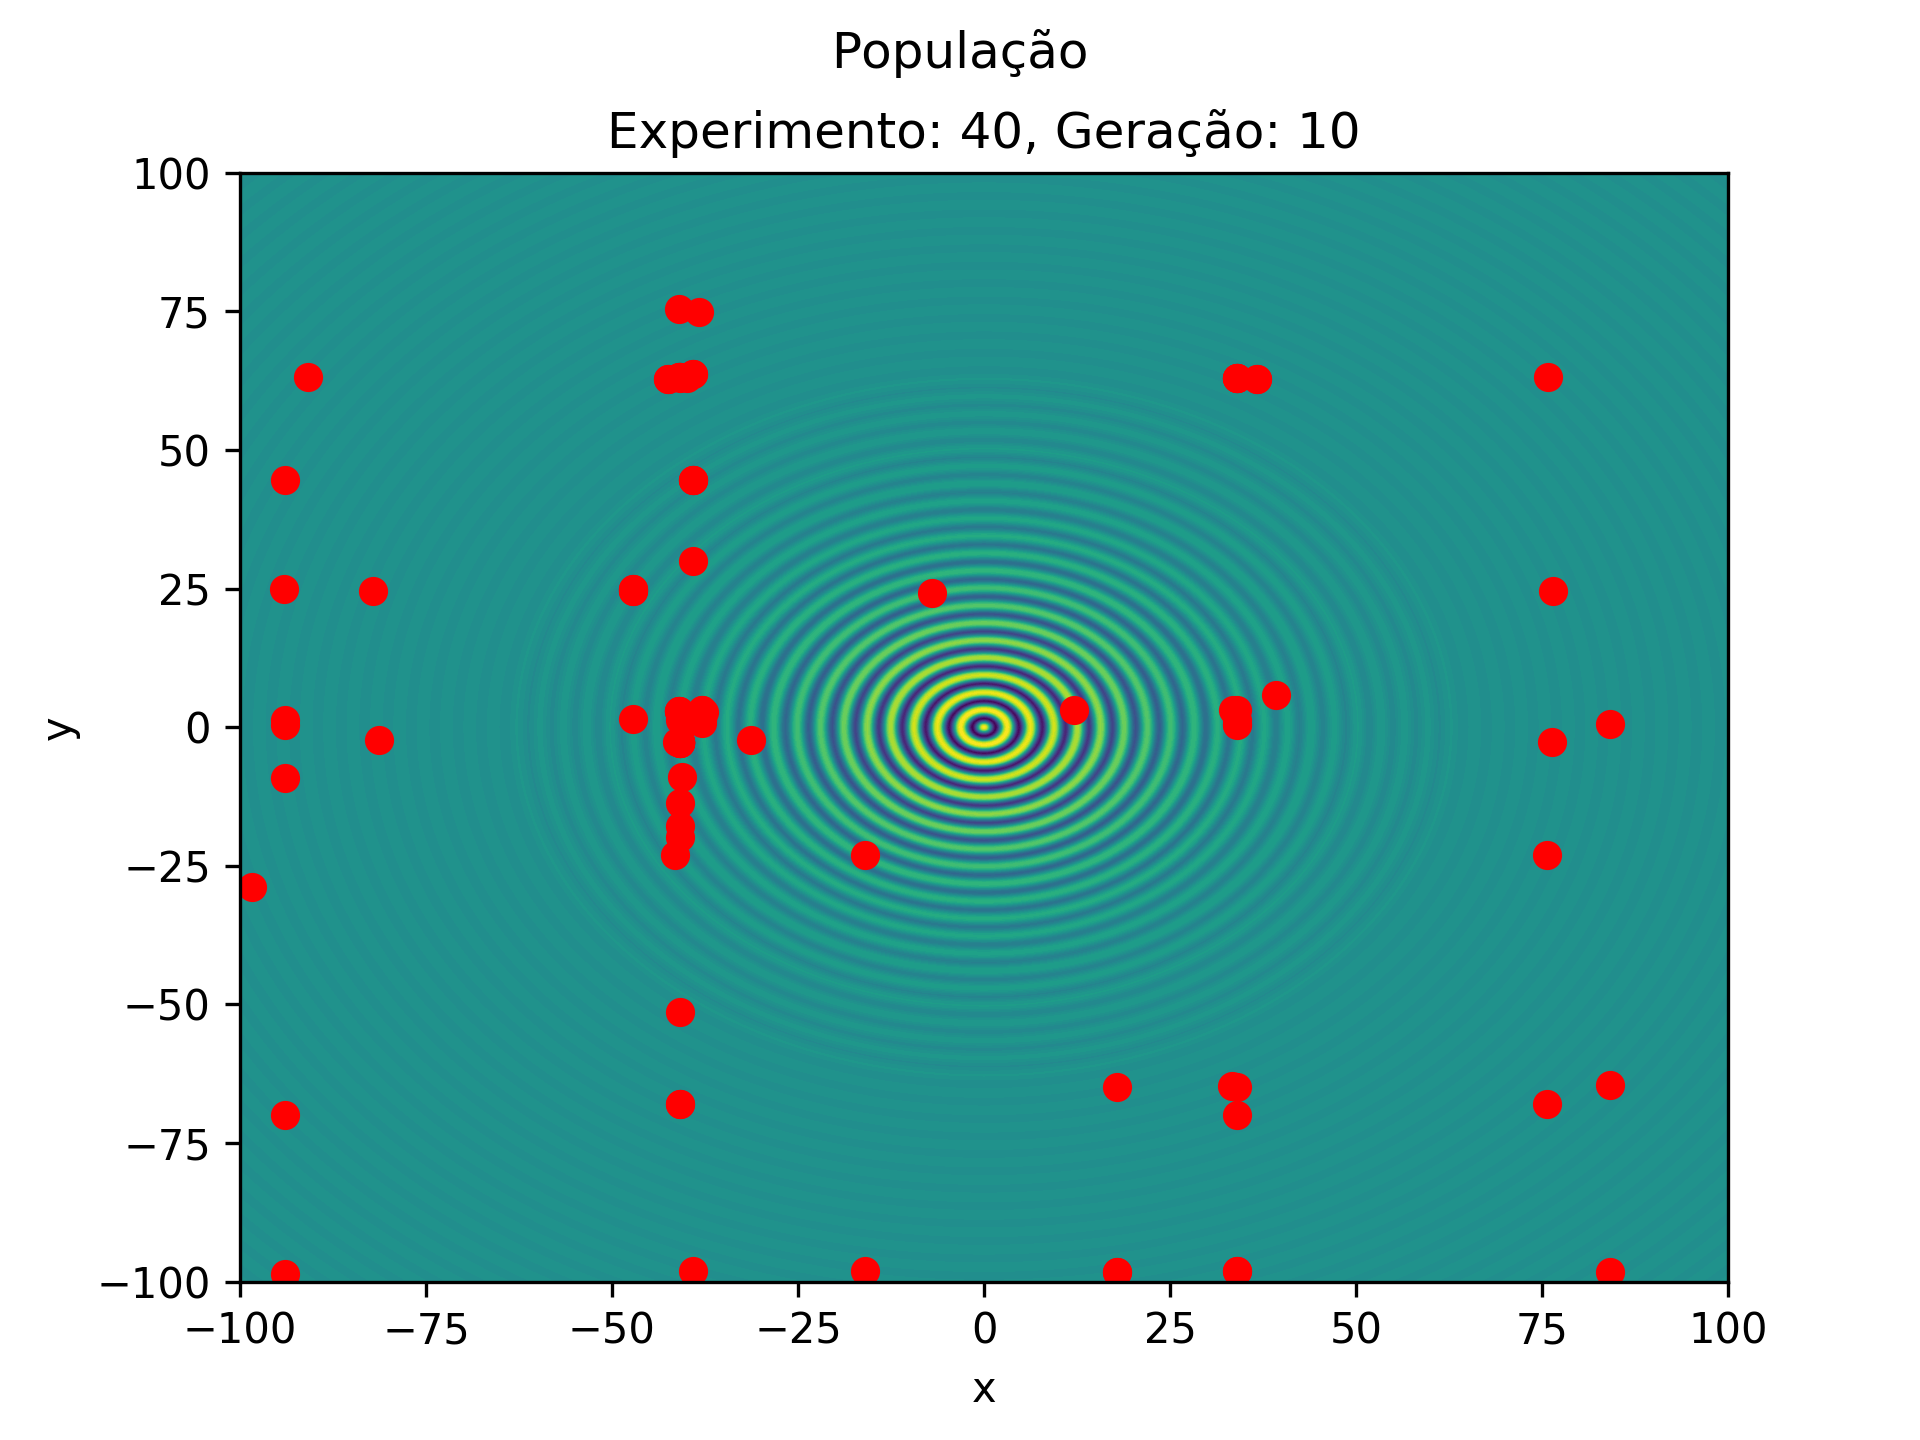
\includegraphics[width=0.9\linewidth]{./imgs/f6_norm_01/population_gen_10_exp_40.png}
		  \end{subfigure}
		  \begin{subfigure}{.5\textwidth}
			\centering
			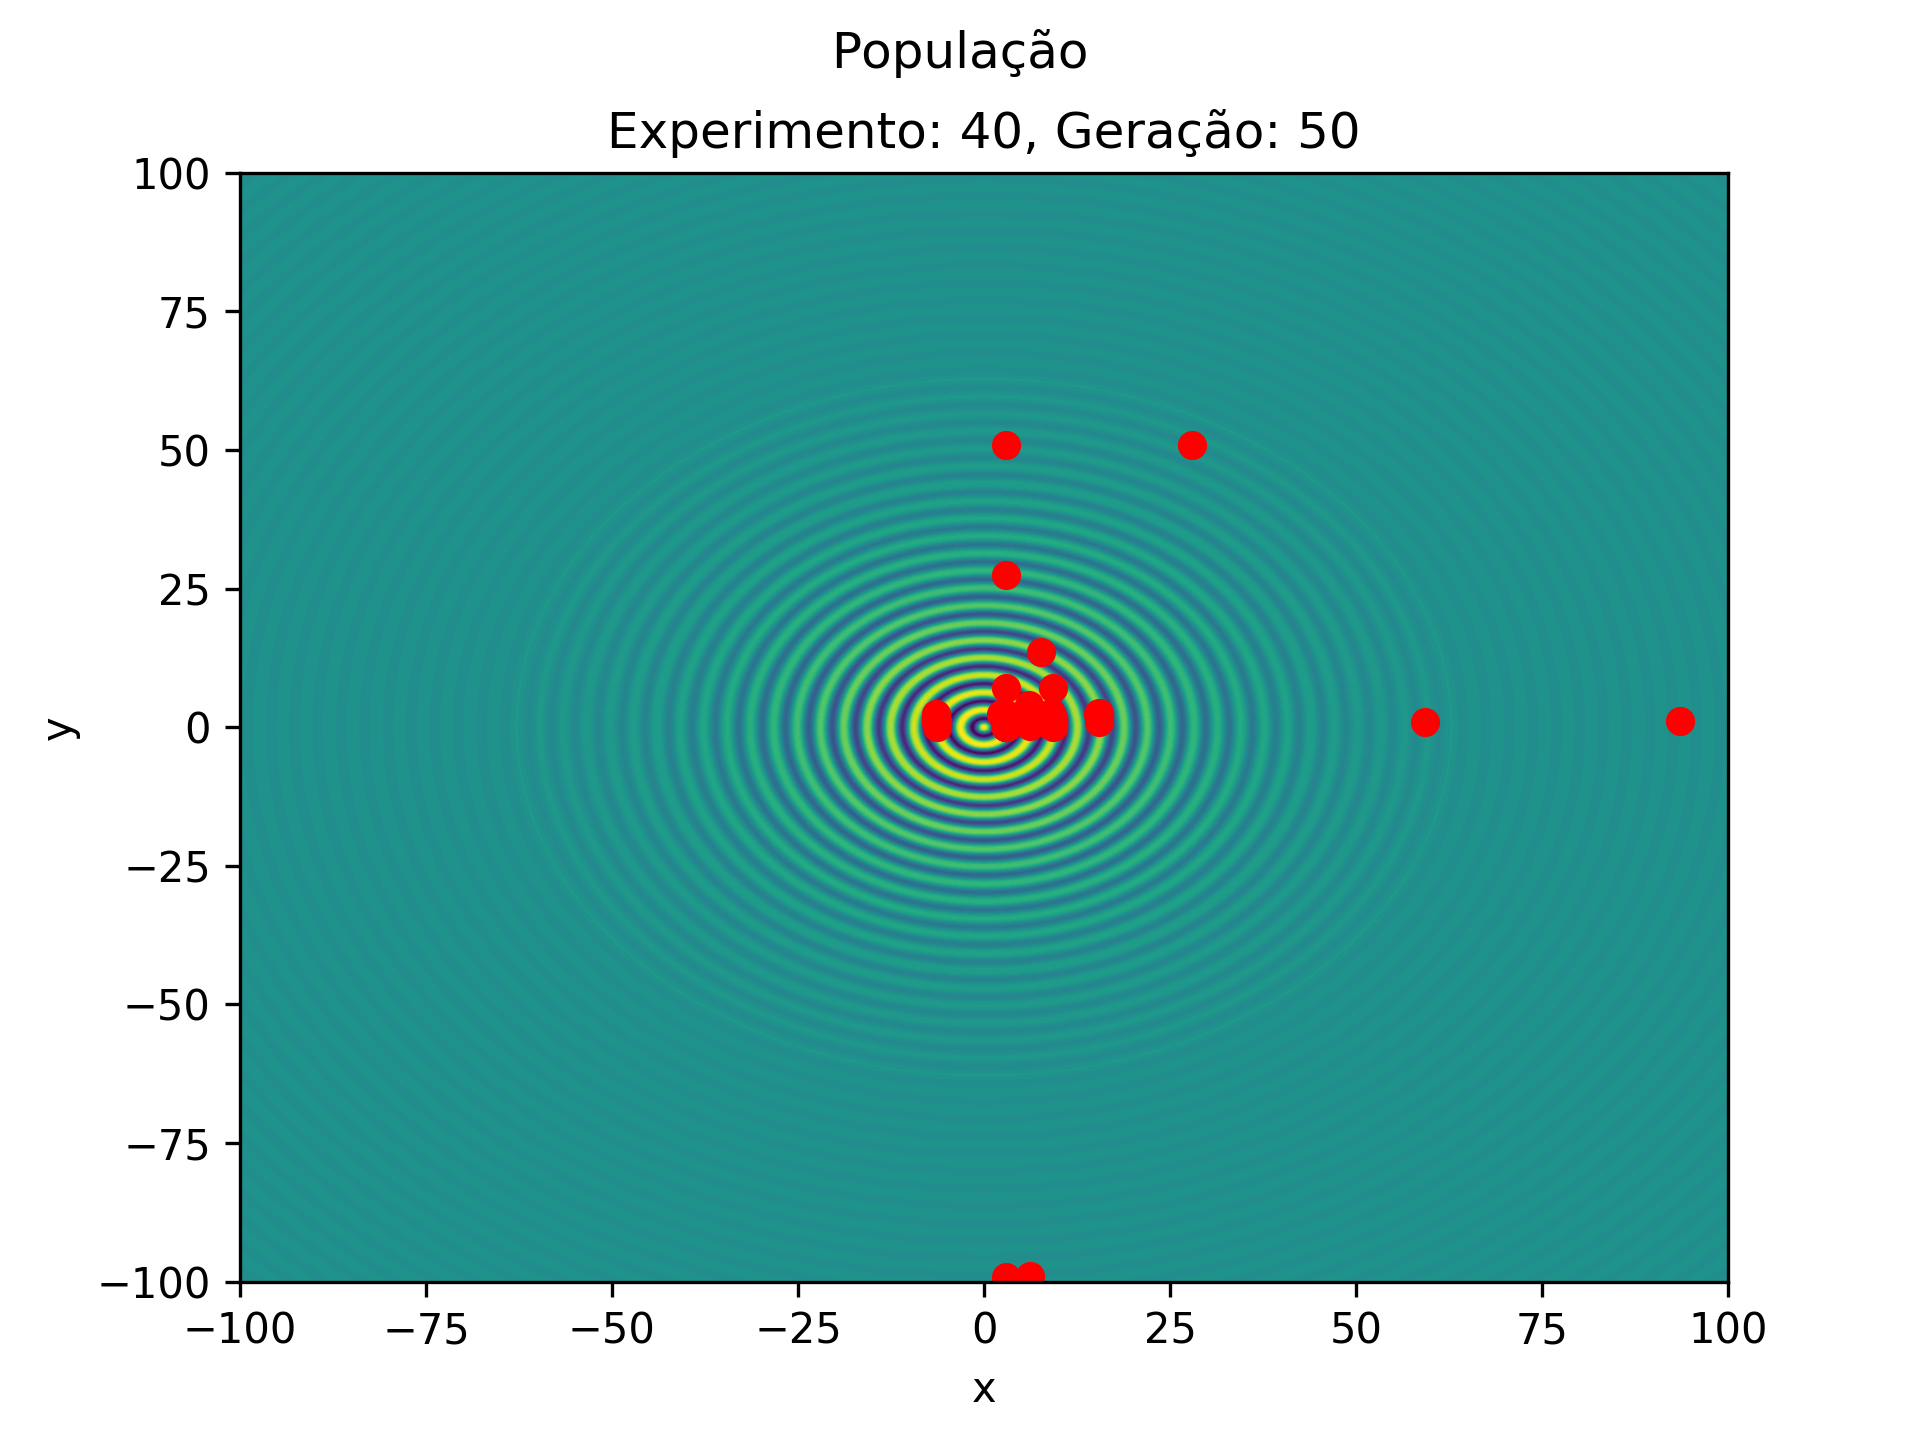
\includegraphics[width=0.9\linewidth]{./imgs/f6_norm_01/population_gen_50_exp_40.png}
		  \end{subfigure}
		  \begin{subfigure}{.5\textwidth}
			\centering
			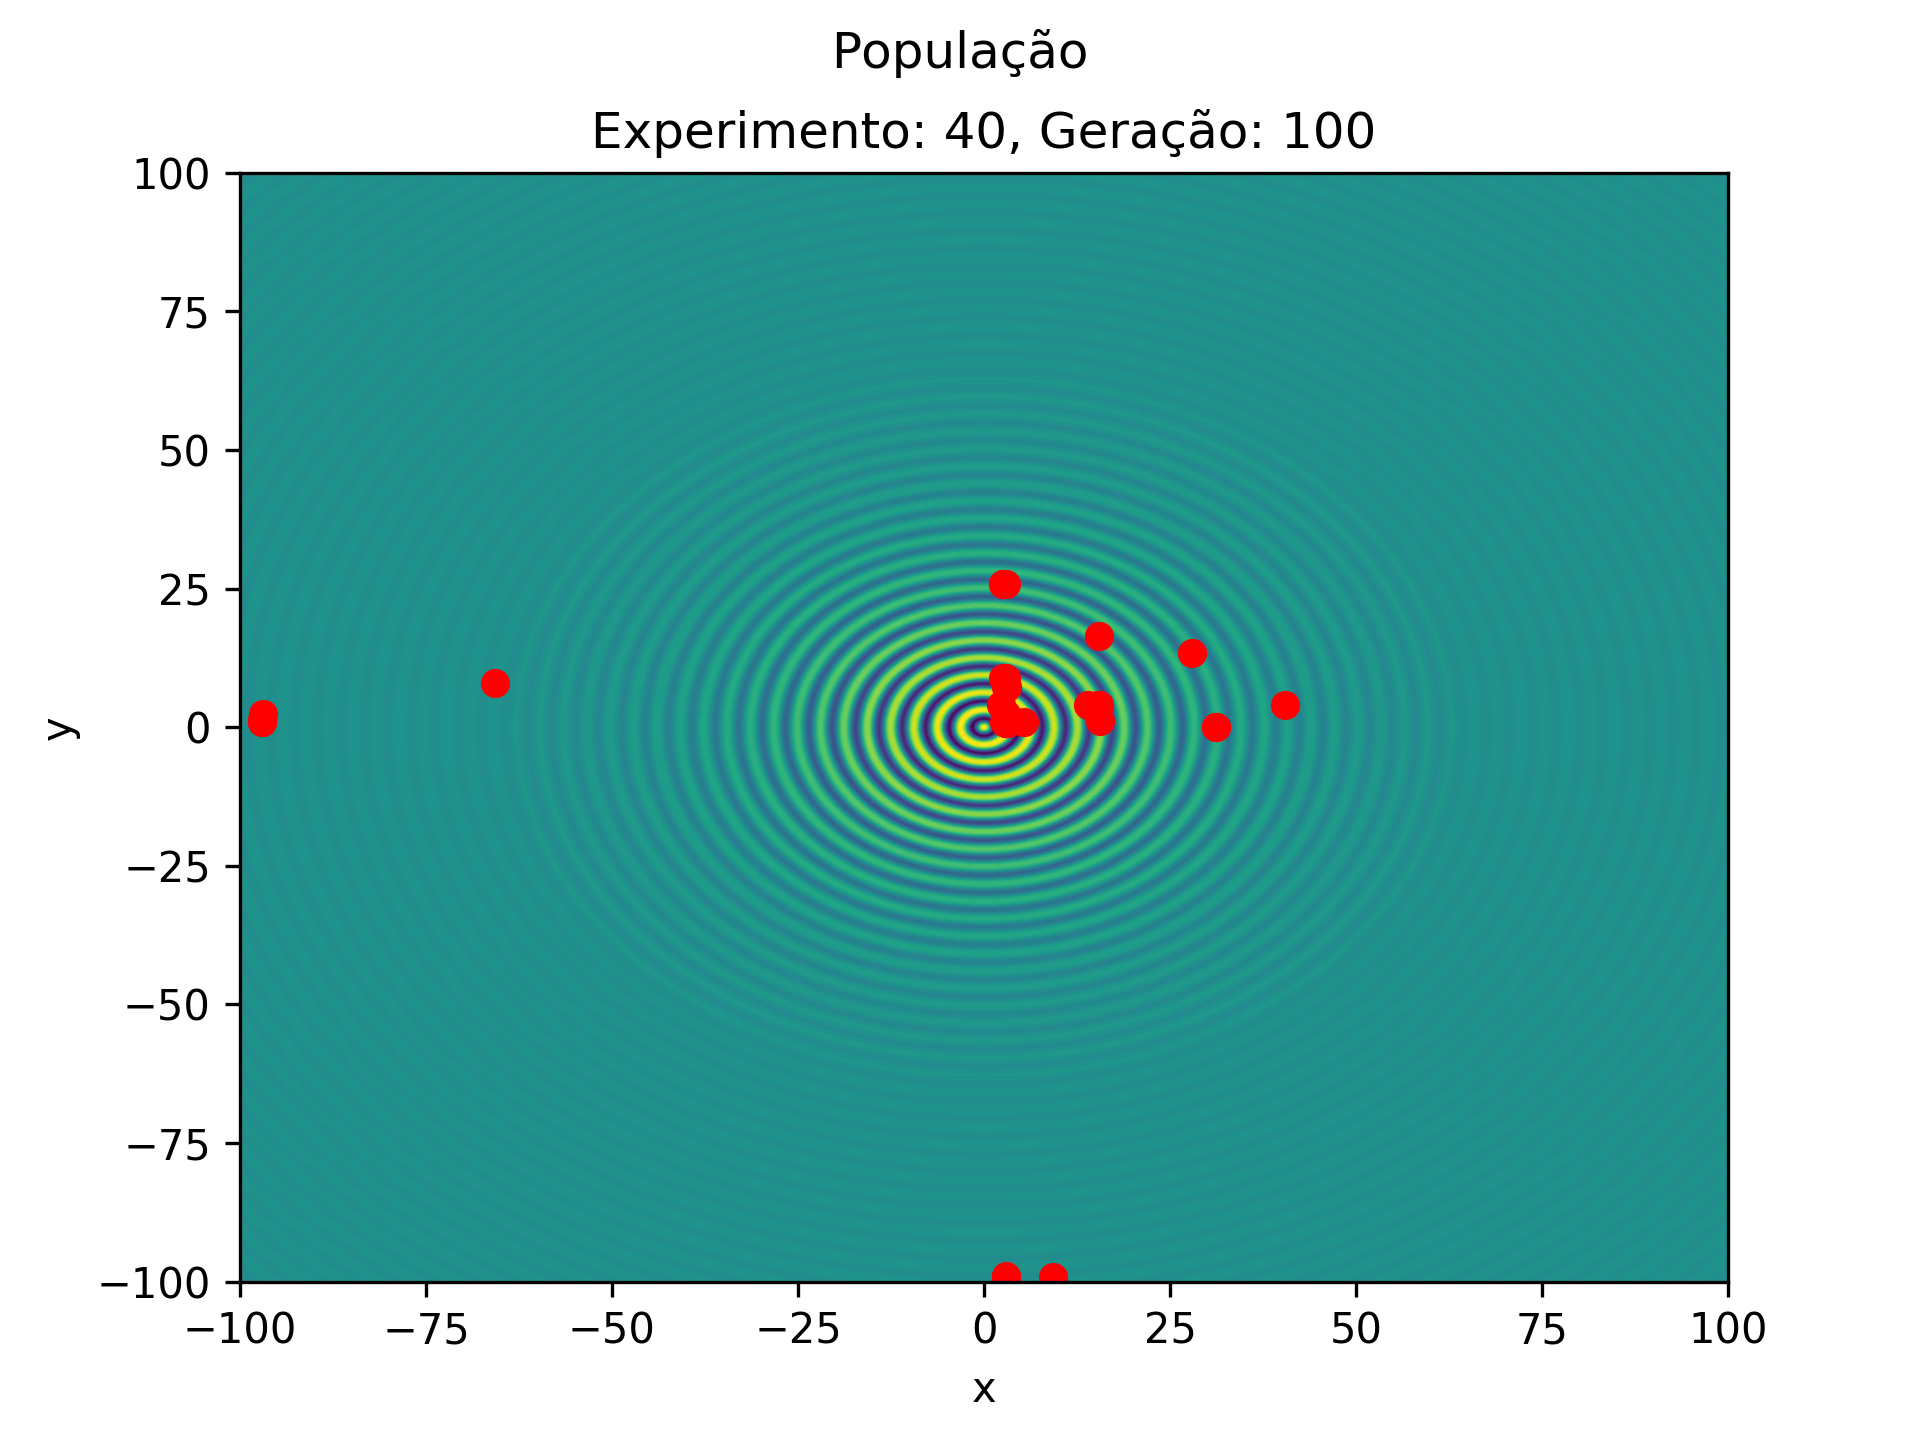
\includegraphics[width=0.9\linewidth]{./imgs/f6_norm_01/population_gen_100_exp_40.png}
		  \end{subfigure}
		\caption{Populações do experimento 40 nas gerações 1, 10, 50 e 100 para o teste número 4 da tabela~\ref{tab:f6_norm_01}}.
		\end{figure}

		\begin{table}[htb]
			\centering
			\begin{tabular}{|c|c|c|c|}
				\hline
				\rowcolor[HTML]{9B9B9B}
				Min & Máx & Média do melhor indíviduo & Média da população \\\hline
				0 & 1 & 999.95860 & 999.82309 \\\hline
				1 & 10 & 999.96781 & 999.76415 \\\hline
				10 & 15 & 999.92180 & 999.51439 \\\hline
				20 & 60 & 999.87967 & 999.56790 \\\hline
			\end{tabular}
			\caption{Resultados usando diferentes valores para o $min$ e $max$ das
			normalização. \label{tab:norm}}
		\end{table}

		Na tabela~\ref{tab:norm} é mostrado os diferentes resultados obtidos quando
		usado diferentes valores para $min$ e $max$.
\end{document}
